
\begin{section}{Simulation Results}
\label{sec:simulation}

% Need to label states of the state vector in the modeling section [x y v \theta]

The case study investigated in this paper is an autonomous unmanned ground vehicle (UGV) navigation under the effects of sensor noise, dynamical changes, and sensor attacks. The vehicle is tasked to travel along a pre-planned trajectory through an obstacle populated environment. 
%We consider a ground vehicle starting at an initial position $\bm{p}(0)=\begin{bmatrix} 0,0 \end{bmatrix}^T$ facing the positive $x$ direction with zero velocity. 
The objective for the UGV is to reach multiple goal points while following a desired trajectory with obstacles of varying distances from the path. The maximum velocity of the vehicle is 3.5m/s and the desired reference velocity is set to 2.5m/s. Three sensors are available to obtain velocity measurements, each with a different level of noise. Throughout the simulation, dynamics are changing affecting the velocity before, during, and after an attack. 




\begin{figure*}[b!th]
%\begin{figure*}[th!]
\begin{tabular}{ccc}

\subfigure[\label{fig:low_noise} ]{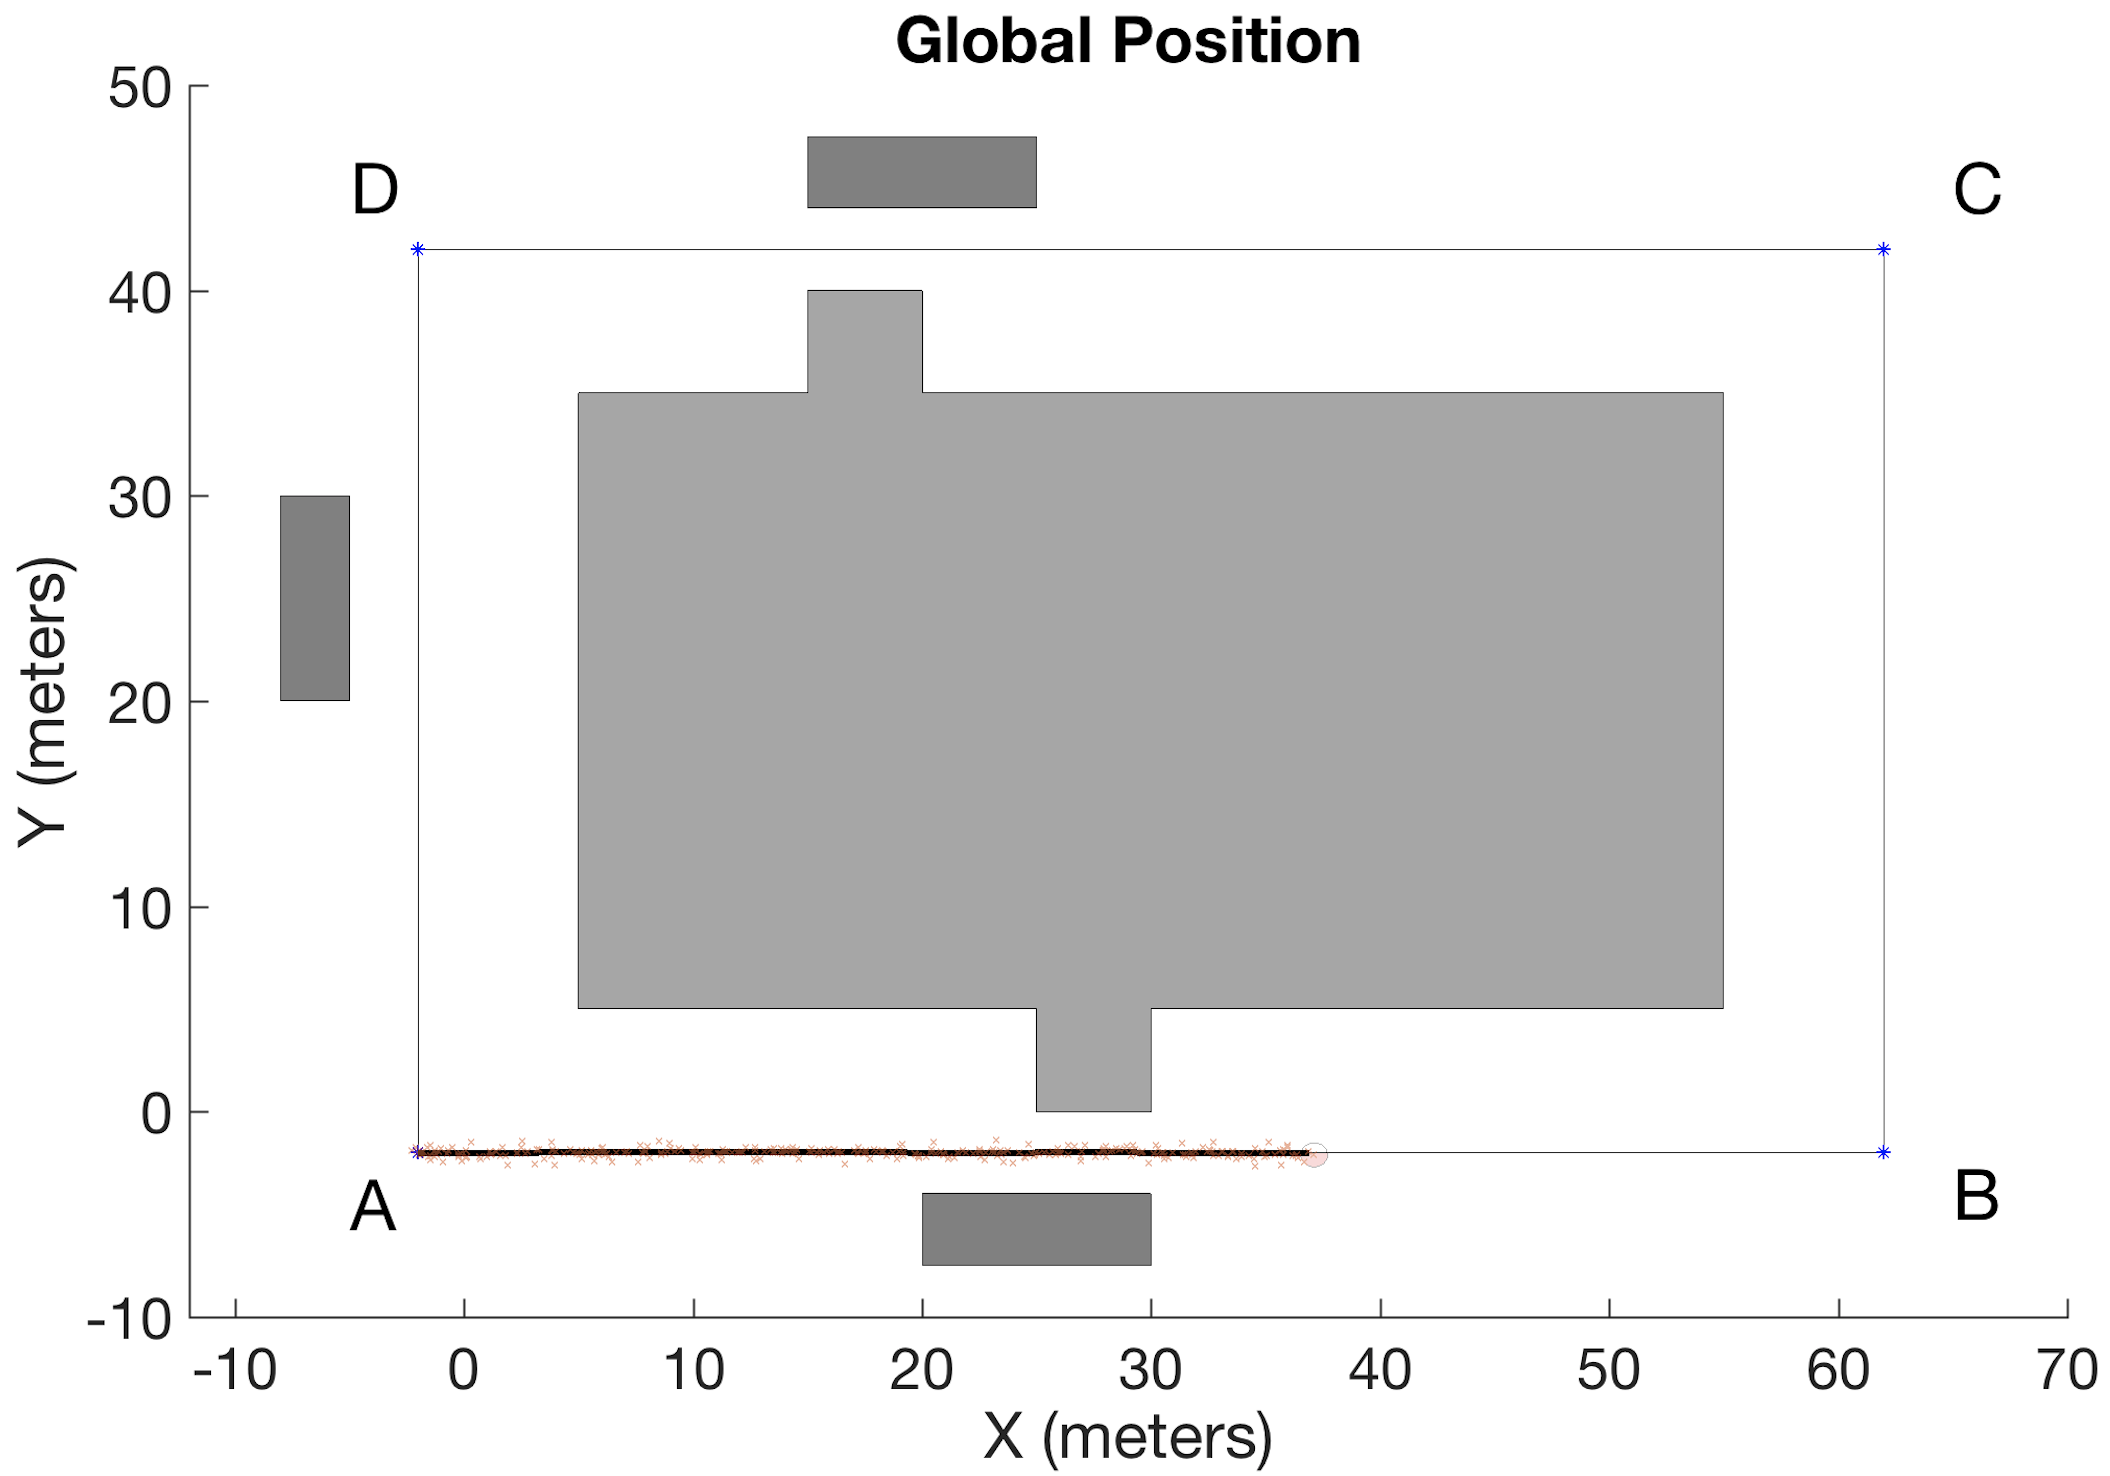
\includegraphics[width = 0.3\textwidth]{Figures/Motion1.png}} &	
\subfigure[\label{fig:low_noise2} ]{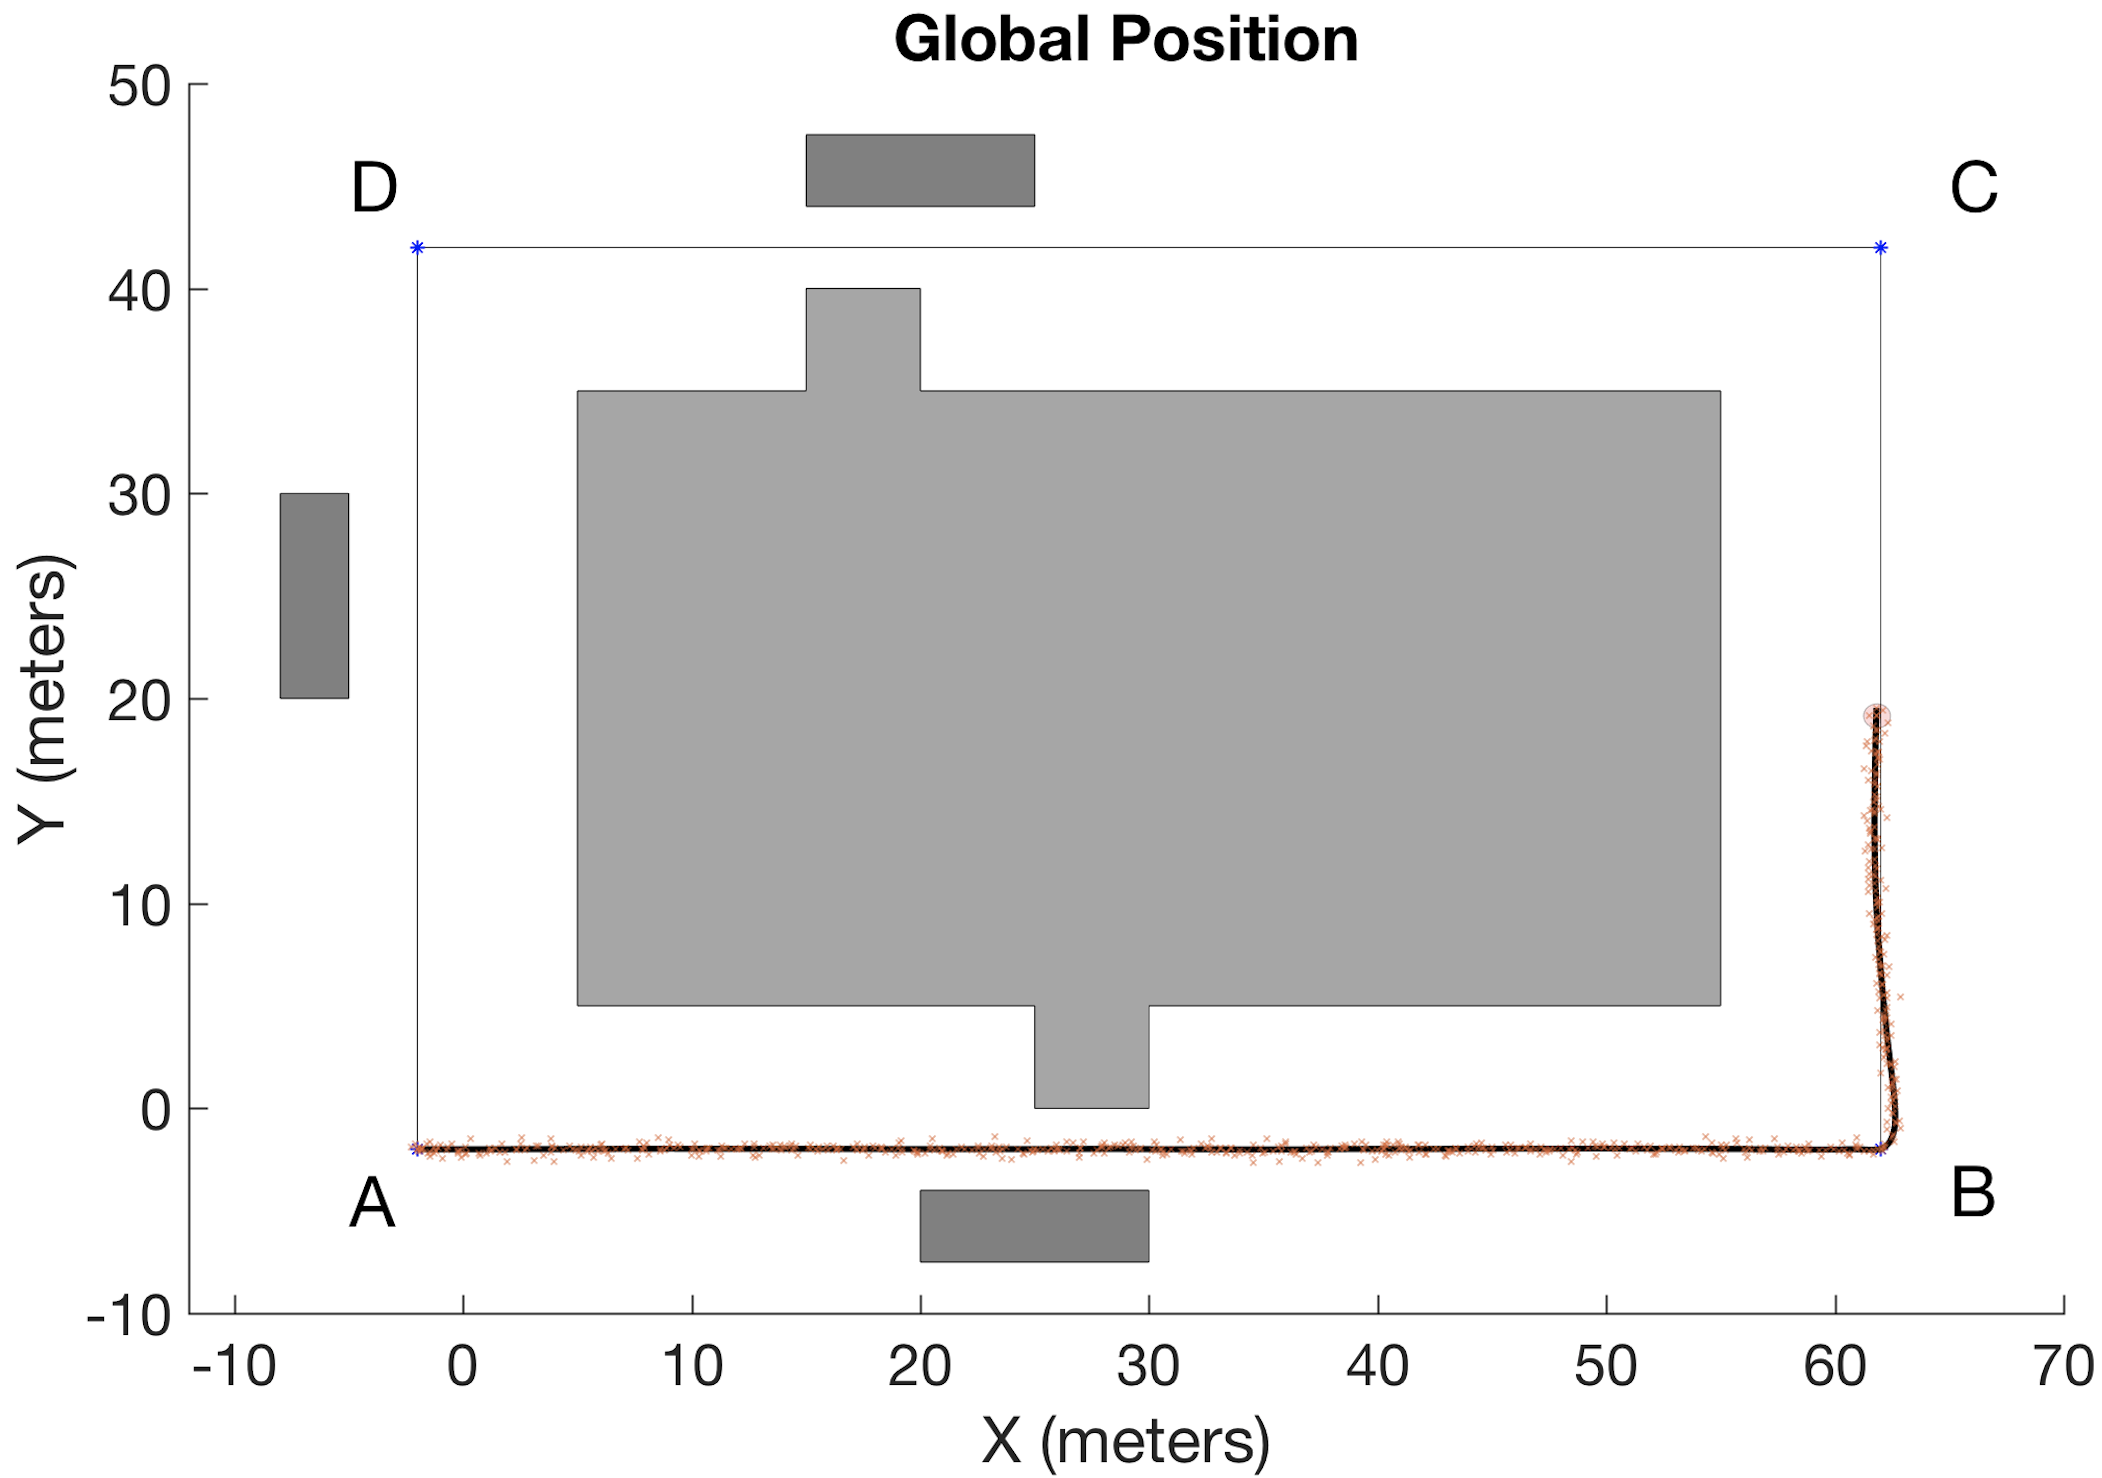
\includegraphics[width = 0.3\textwidth]{Figures/Motion2.png}} &
\subfigure[\label{fig:at_attack} ]{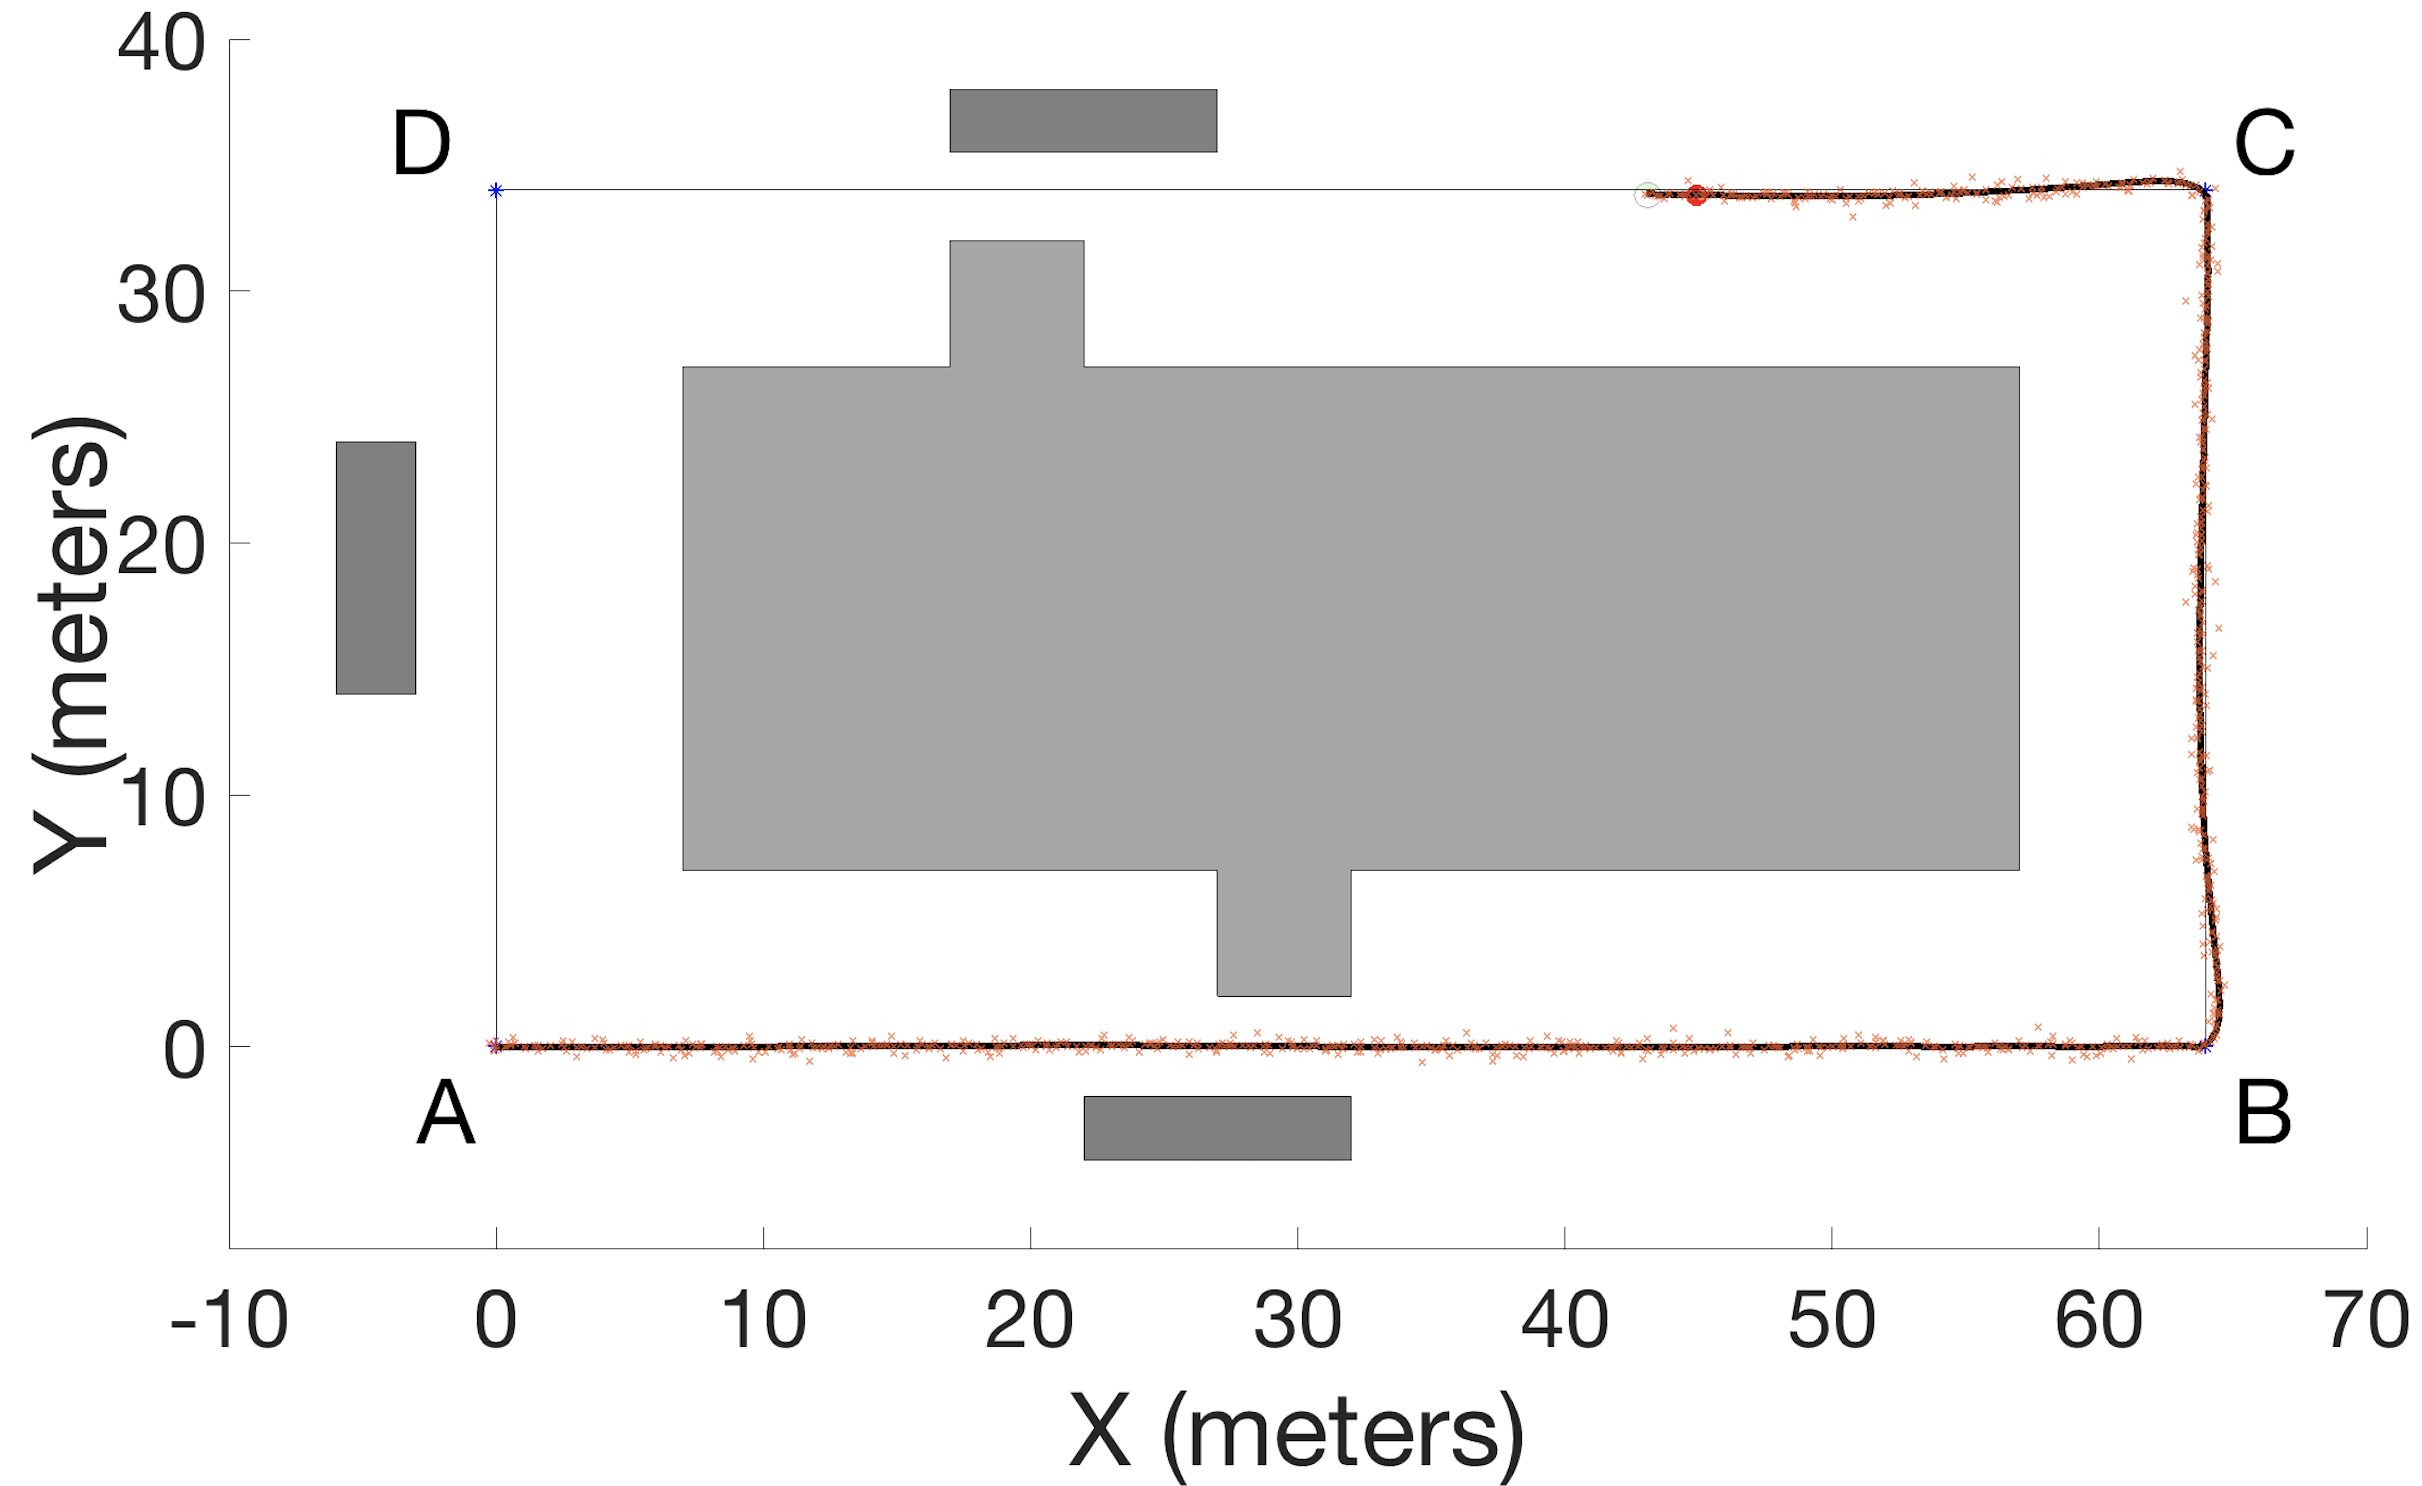
\includegraphics[width = 0.3\textwidth]{Figures/Motion3.png}}
\end{tabular} \\
\begin{tabular}{ccc}
\subfigure[\label{fig:after_detection} ]{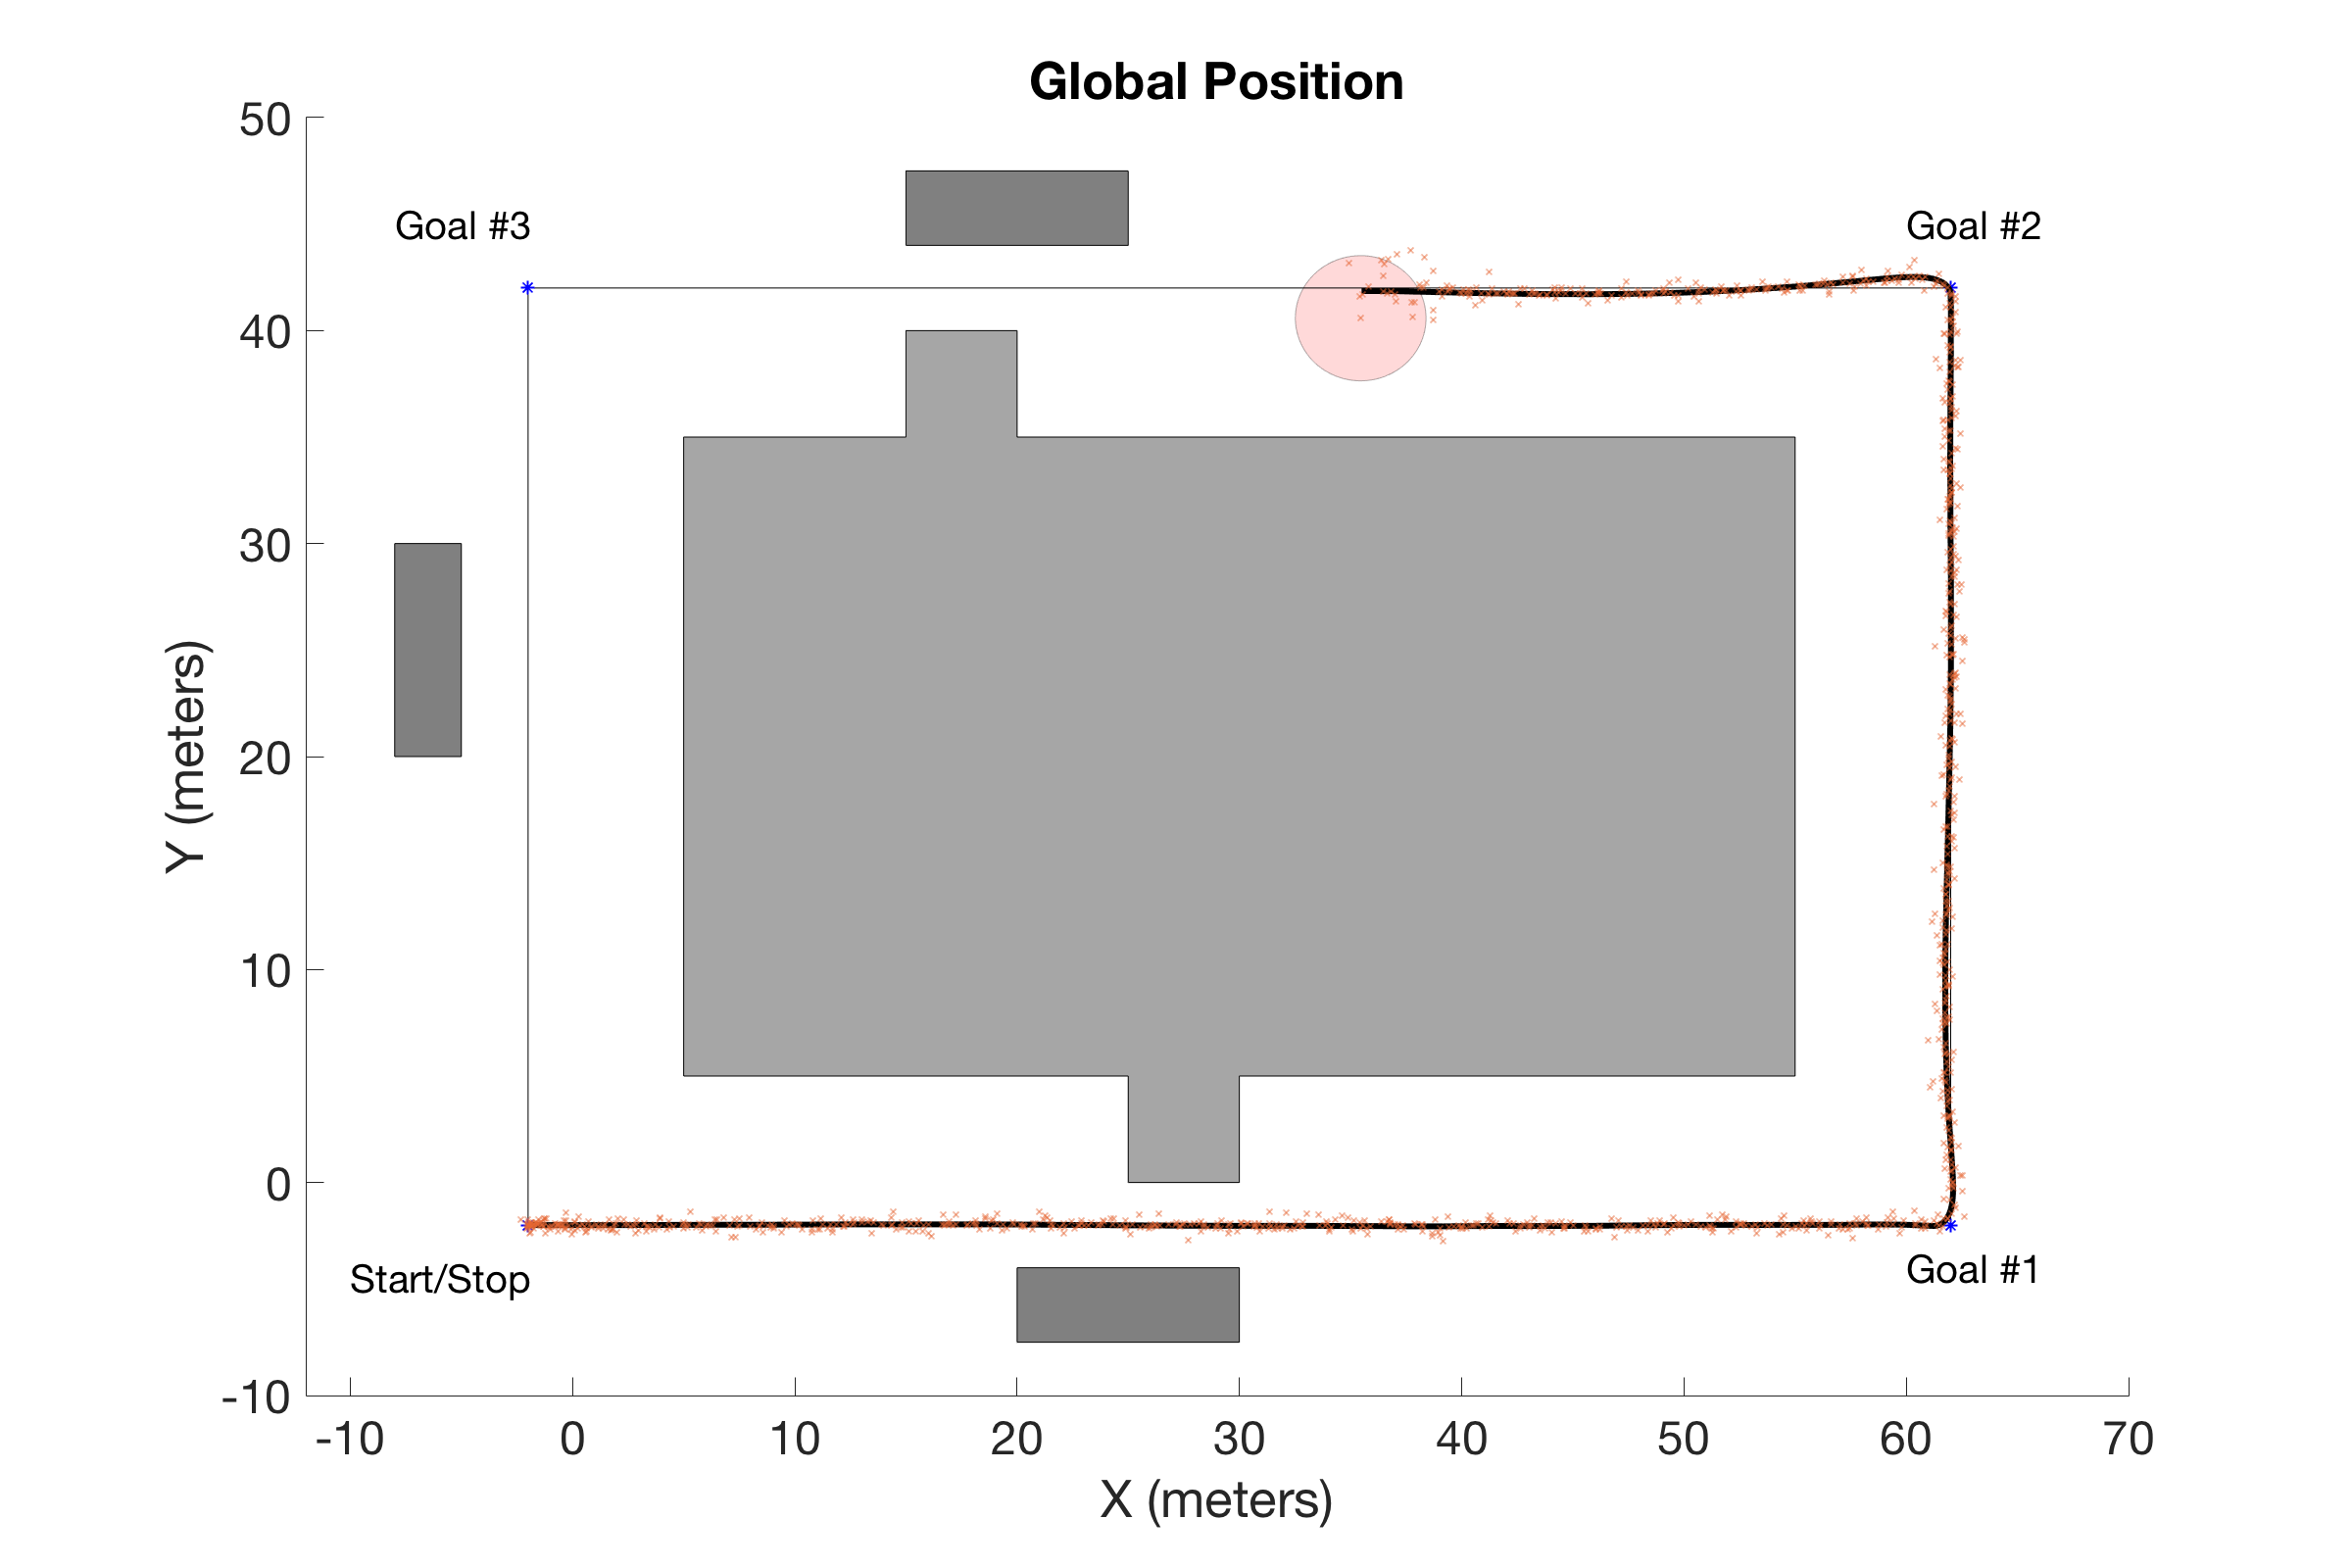
\includegraphics[width = 0.3\textwidth]{Figures/Motion4.png}} &
\subfigure[\label{fig:adapt_region} ]{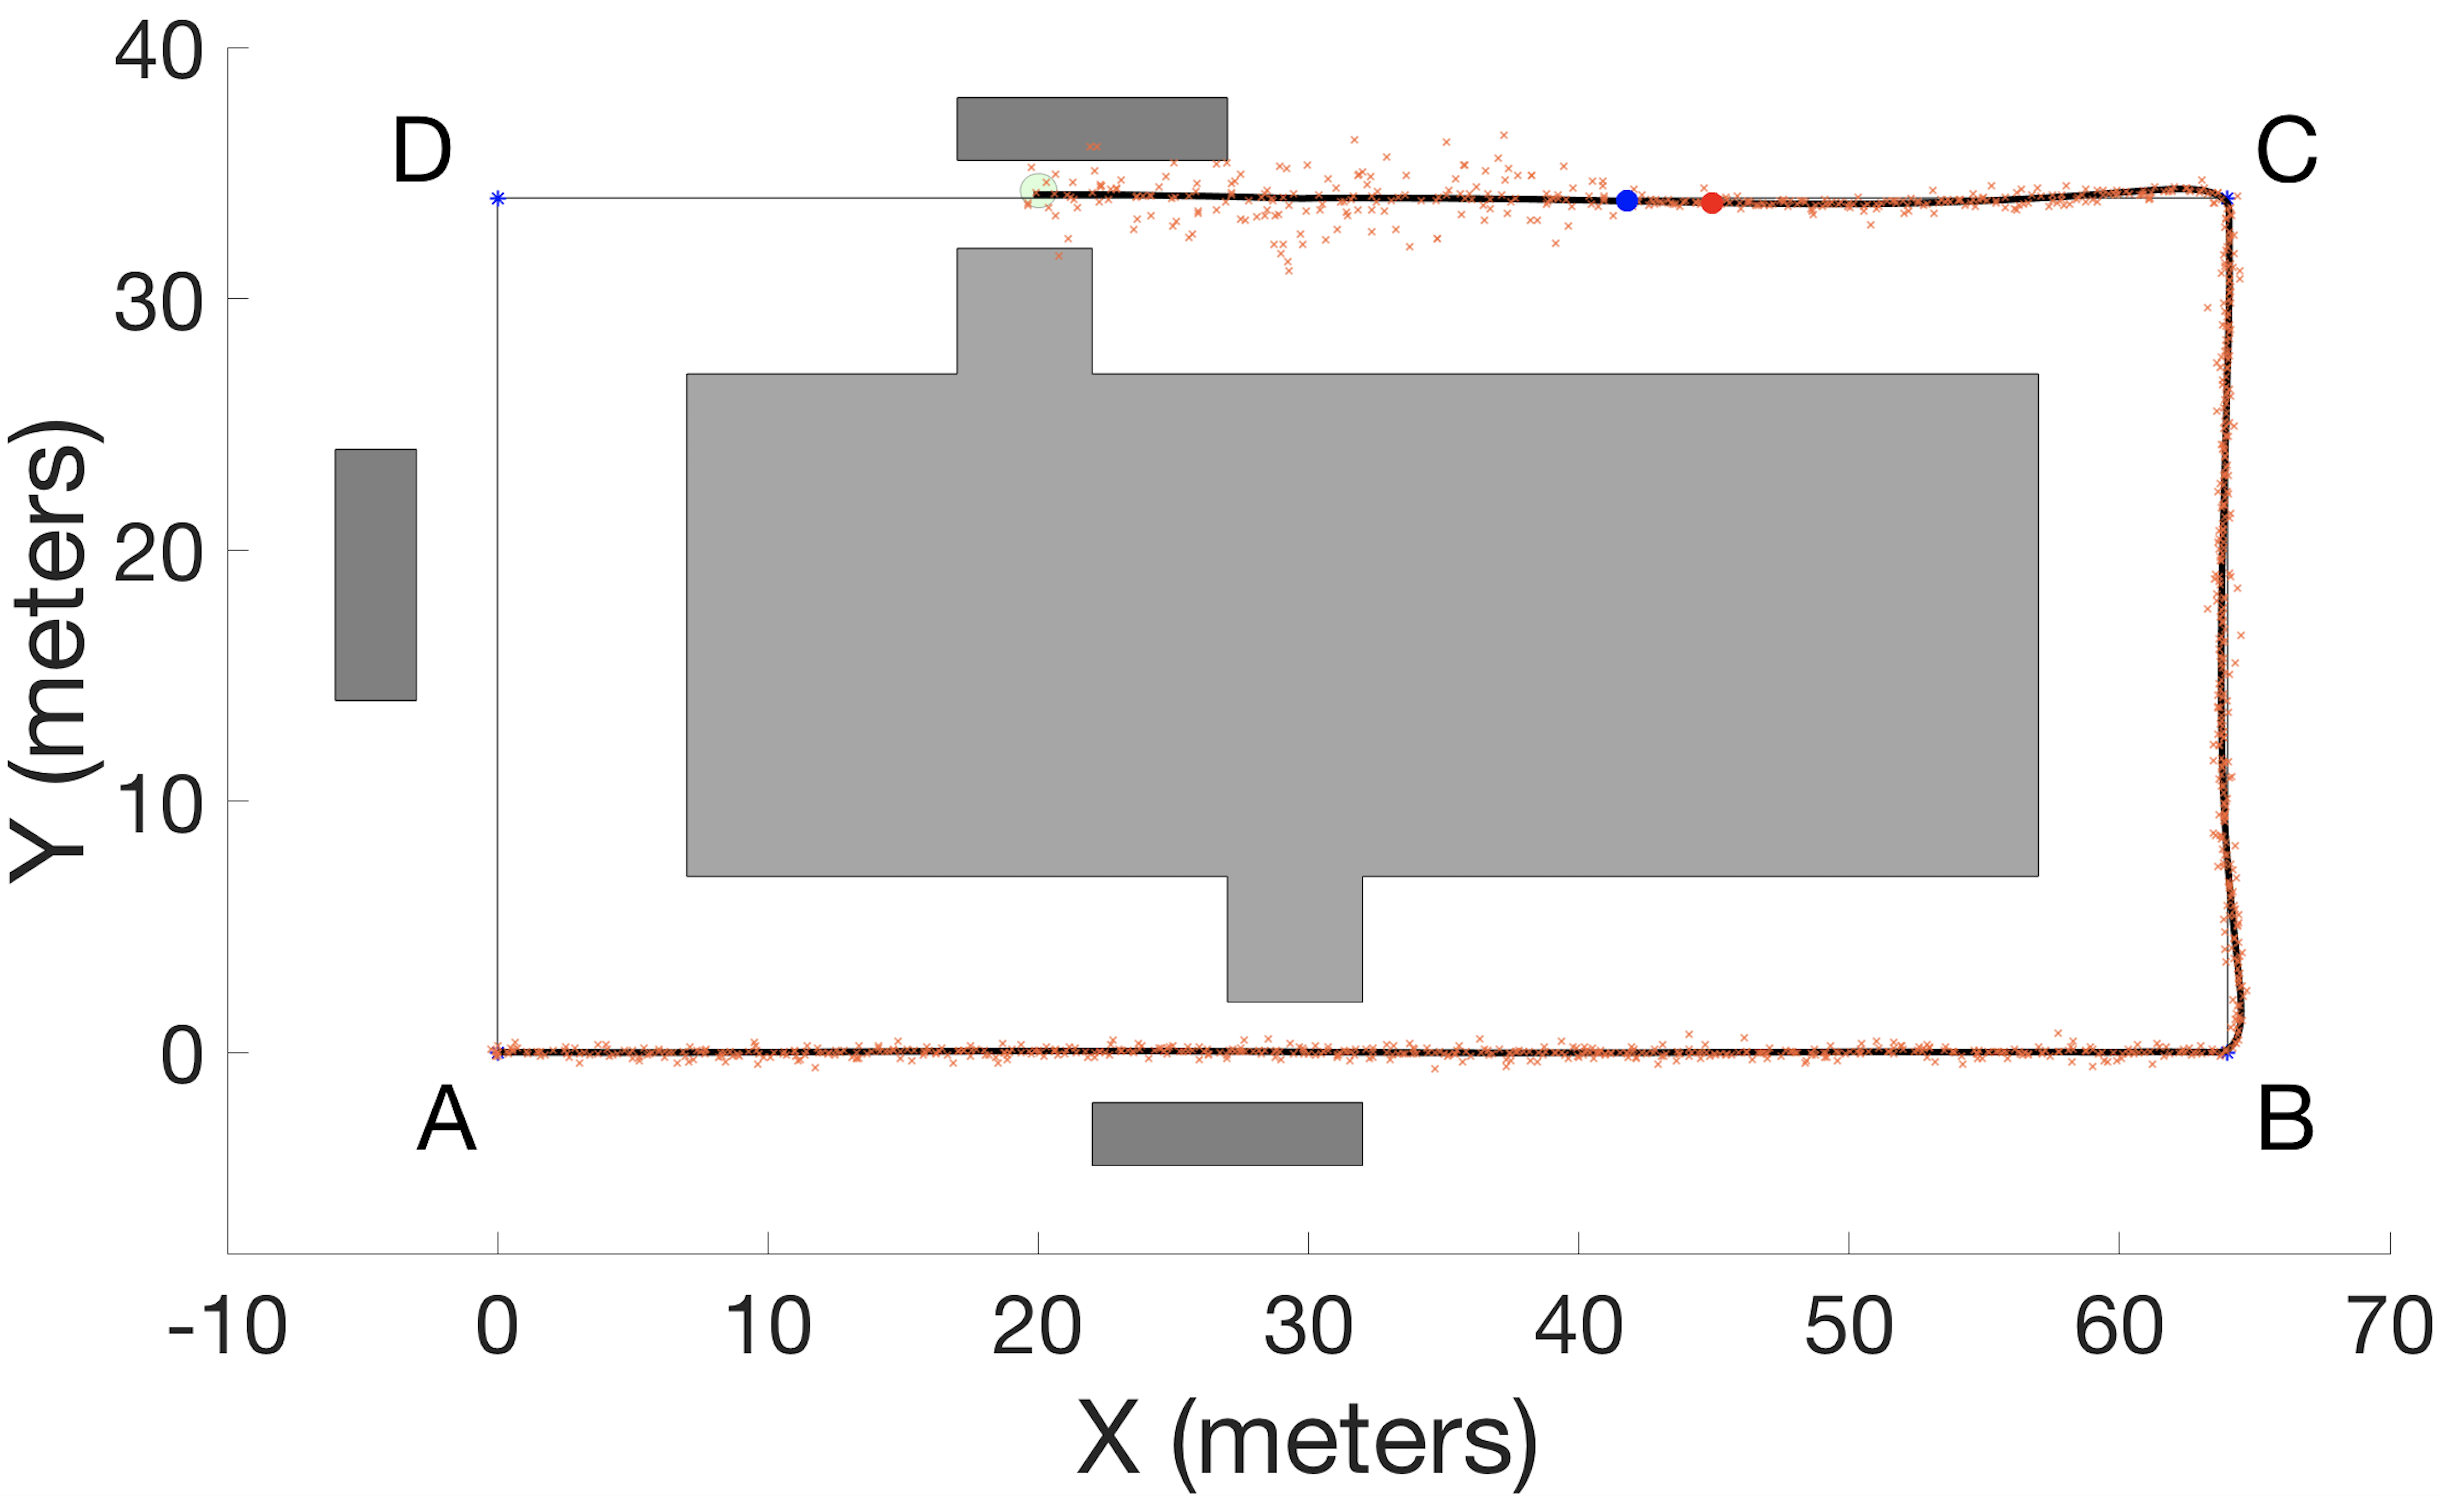
\includegraphics[width = 0.3\textwidth]{Figures/Motion5.png}} & 
\subfigure[\label{fig:continue_motion} ]{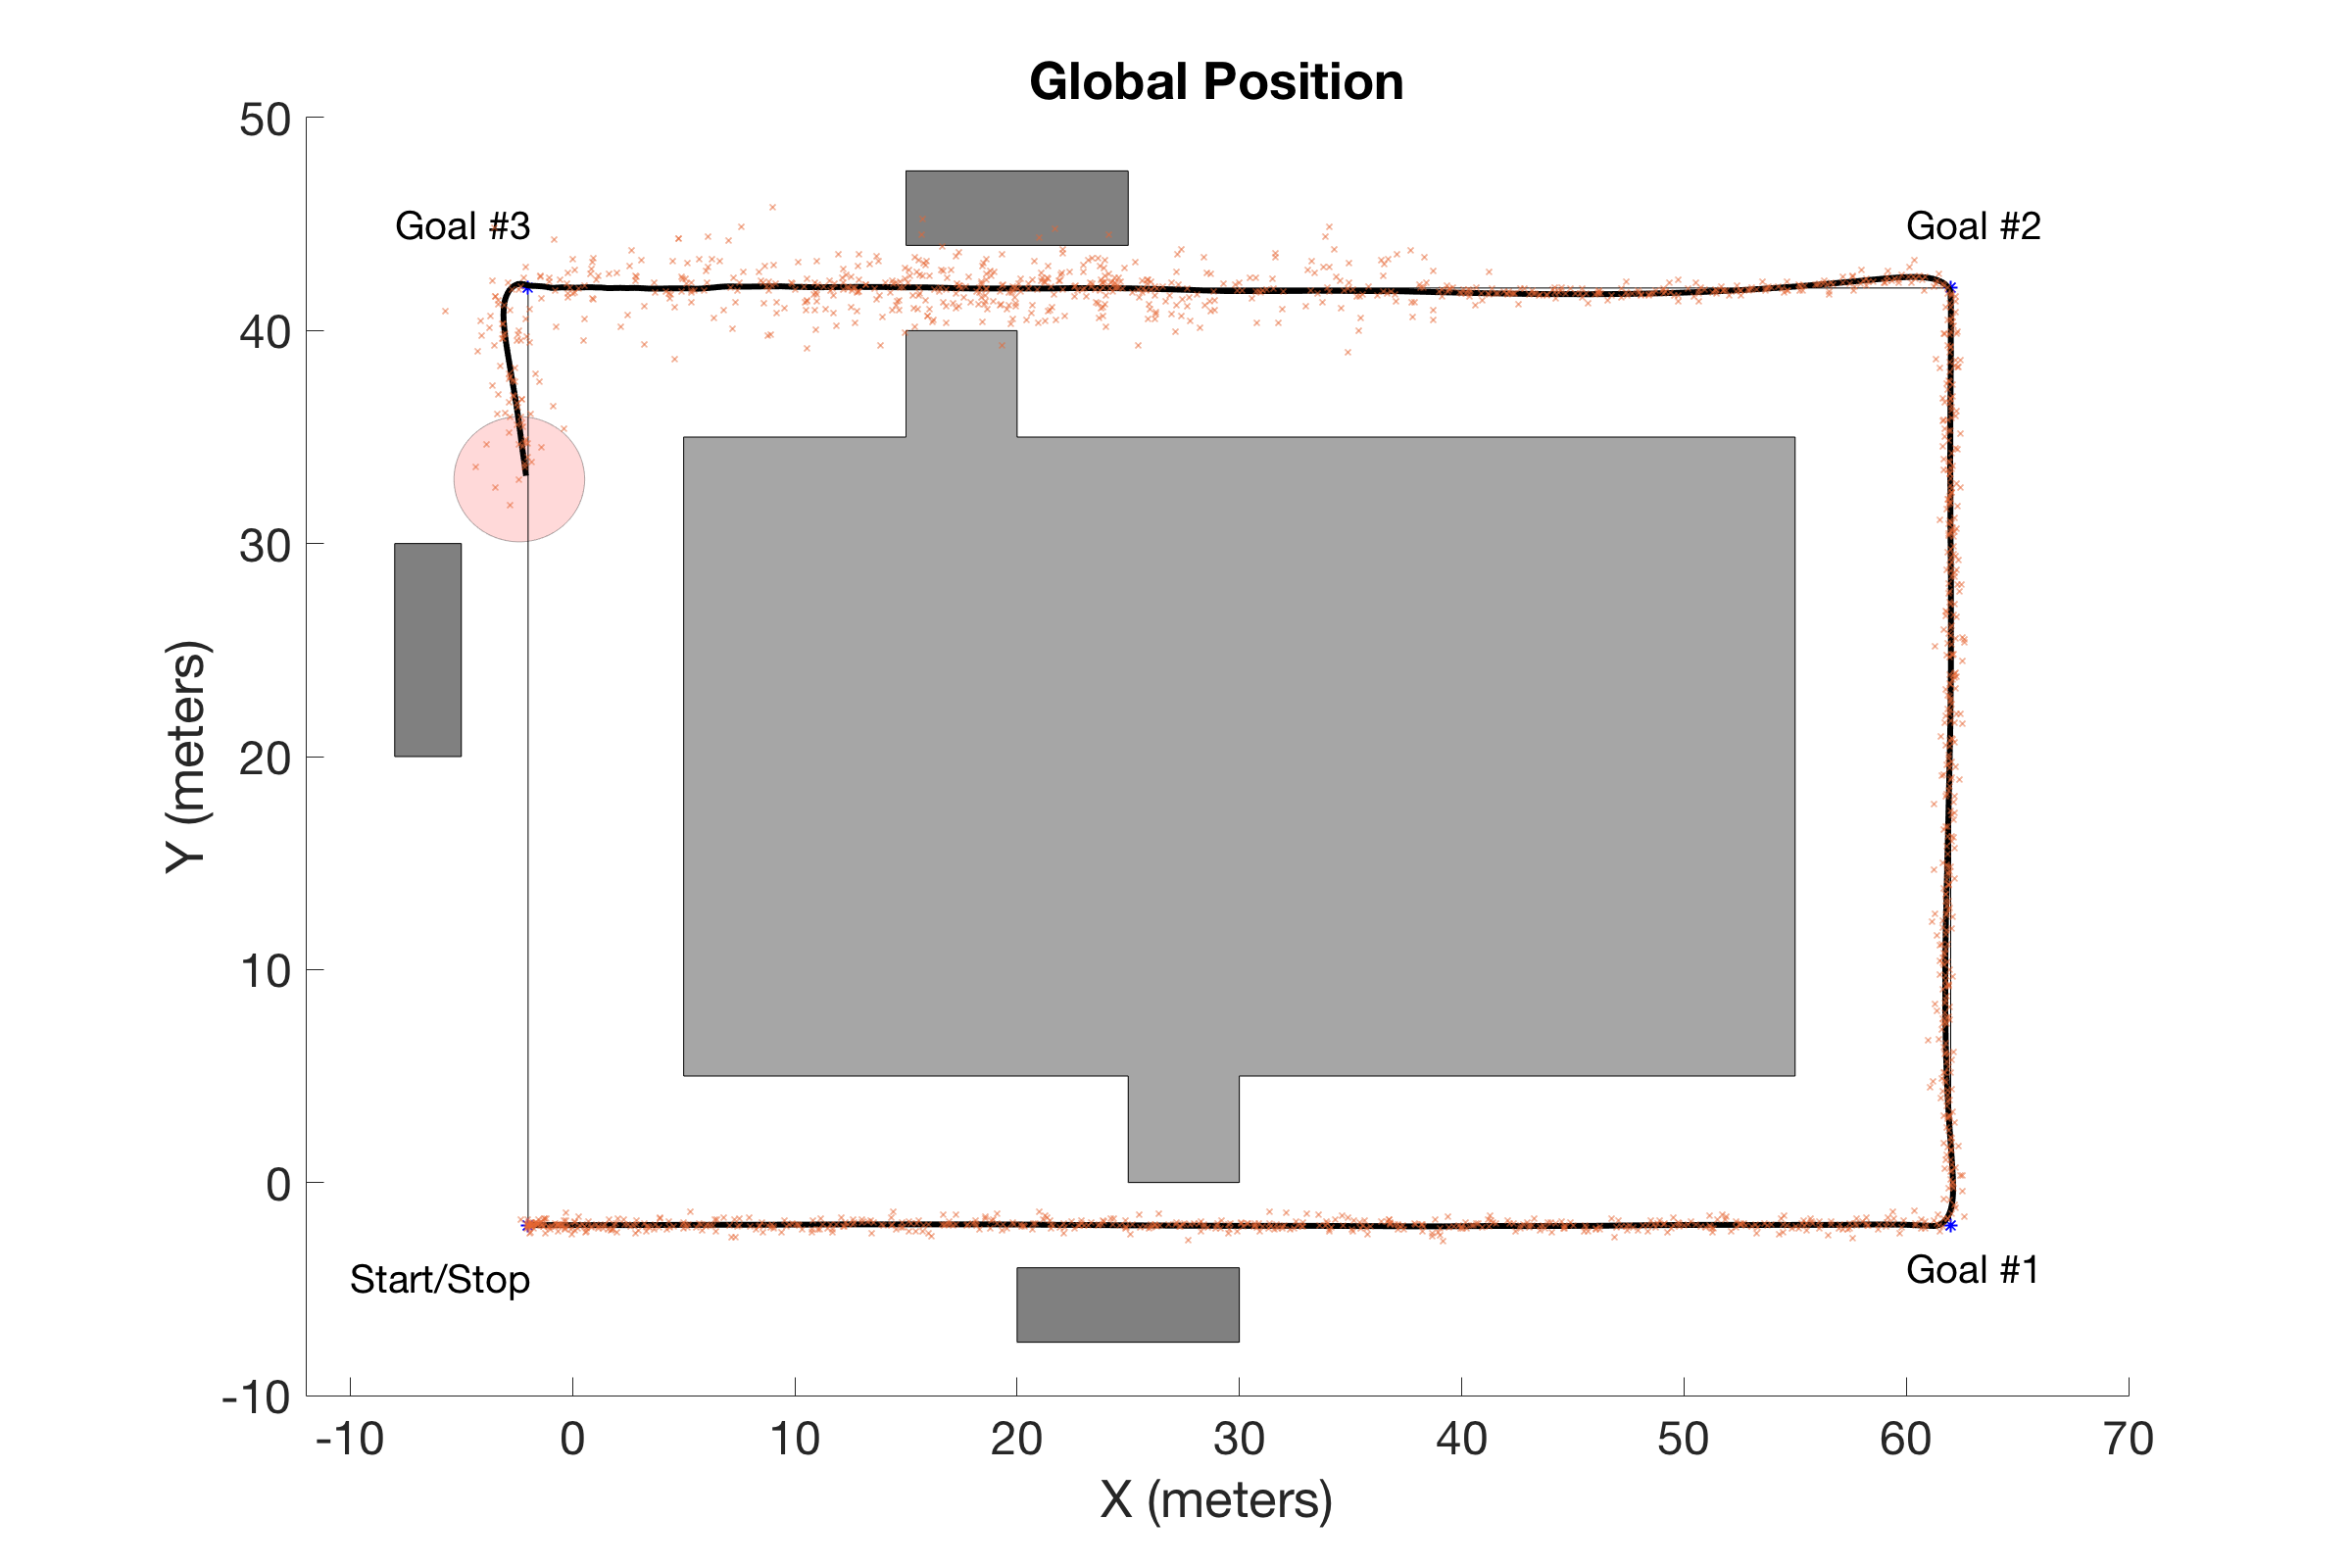
\includegraphics[width = 0.3\textwidth]{Figures/Motion6.png}}

\end{tabular}
\caption{A comparison in time of a vehicle navigating through an obstacle filled environment. In (a),(b), and (c) the measurement set is uncompromised and the system is only experiencing dynamical changes. Subfigures (d),(e), and (f) are post detection of a sensor attack where the sensor has been removed from the measurement set. Uncertainty is increased with the smaller sensor set, now the vehicle adapts the velocity as it approaches obstacles.}

\end{figure*}

In Figure \ref{fig:low_noise}, the vehicle is moving along the trajectory with no compromised sensors and far from obstacles. The confidence region is, small in this case because all sensors are available and fused togetehr. 
%Velocity is unaltered due to the obstacles being well outside the uncertainty boundaries.

While all sensors are uncompromised, Figure \ref{fig:low_noise2} shows a region where the vehicle is undergoing dynamical changes. The confidence region remains unchanged due to the full uncompromised set of sensors. The adaptive controller is maintaining a reference velocity, even while system dynamics are changing.

Figure \ref{fig:at_attack} shows vehicle position at the starting time of the ramped sensor attack. The amplitude of the attack is still well within the sensor noise bounds, detection does not occur.


Detection of the spoofed sensor is demonstrated in Figure \ref{fig:after_detection}. The spoofed sensor has been removed from the system, leaving a smaller set of available sensors with higher uncertainty. The confidence region grows in size due to the changes in uncertainty. Obstacles are still well outside of the bounds, allowing the vehicle to continue navigating at its desired velocity.

Figure \ref{fig:adapt_region} shows the confidence region shrinking in size when the vehicle navigates near obstacles of closer distances. More data points are used to improve this estimation, while the velocity is reduced to lessen uncertainty while moving.

Once the vehicle is past the obstacles that are at close distances, shown in Figure \ref{fig:continue_motion}, the vehicle is able to move freely again at its desired velocity. The confidence region remains at a much larger radius due to the smaller set of available sensors.

% \begin{figure}
% \vspace{1pt}
% %\centering
% 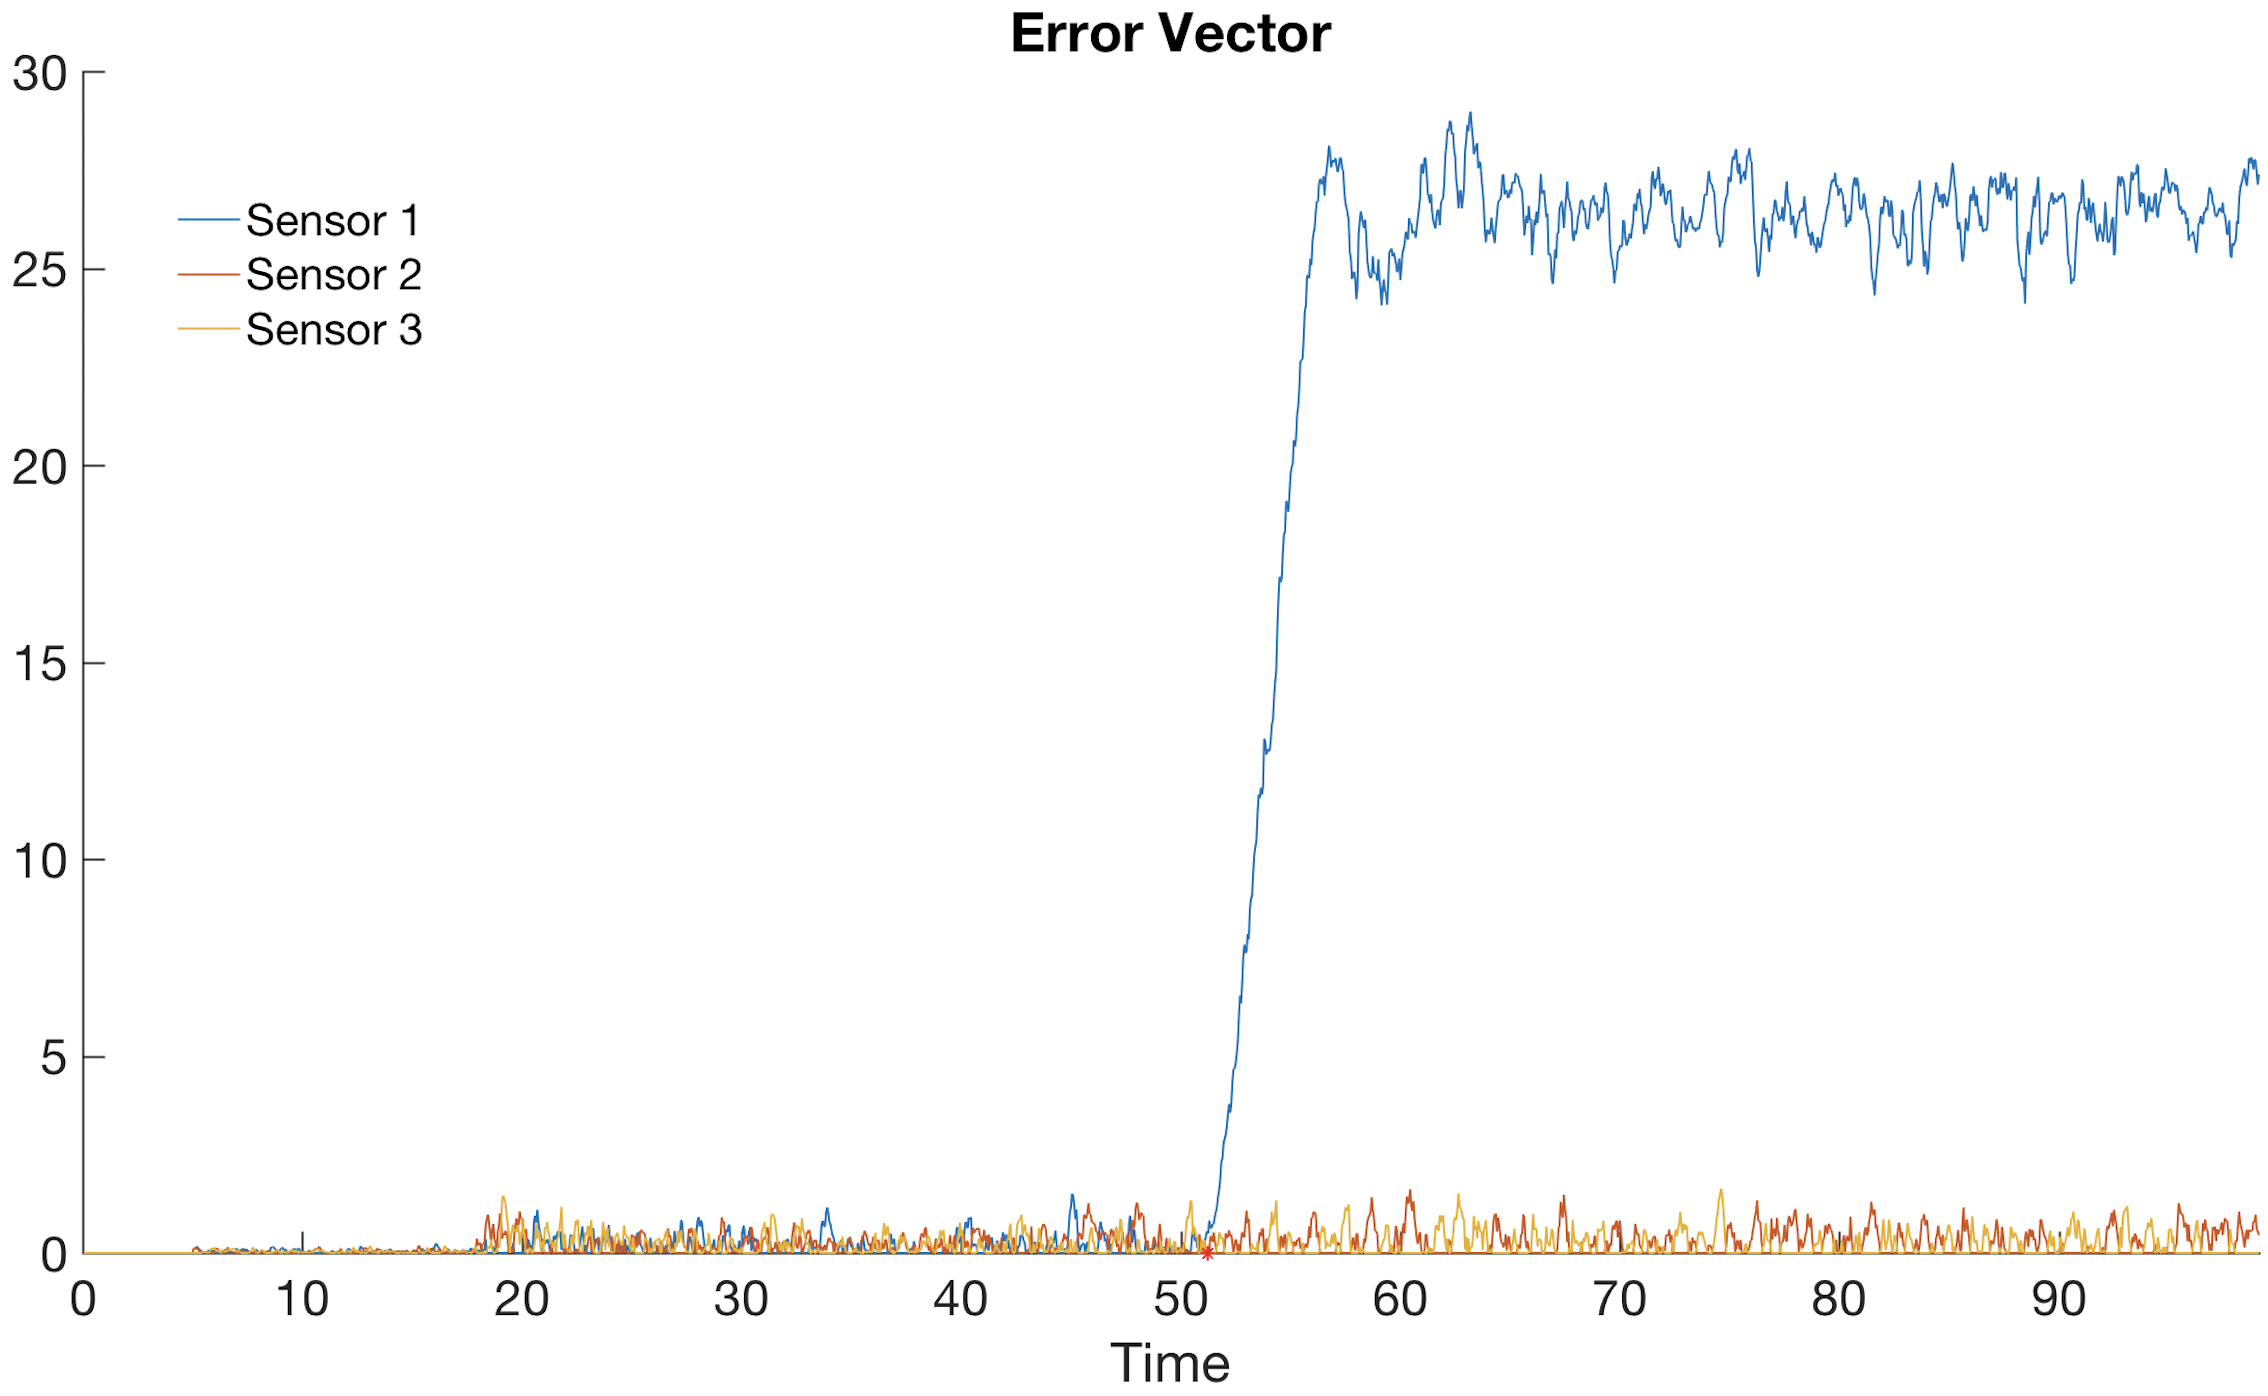
\includegraphics[width=0.48\textwidth]{Figures/Error_vector.png}
% \caption{The error vector is computing magnitudes of error for each of the sensors. As a sensor's error reaches a threshold, the sensor will be removed from the system.}
% \label{fig:sensor error}
% \end{figure}

\begin{figure}[ht!]
\centering
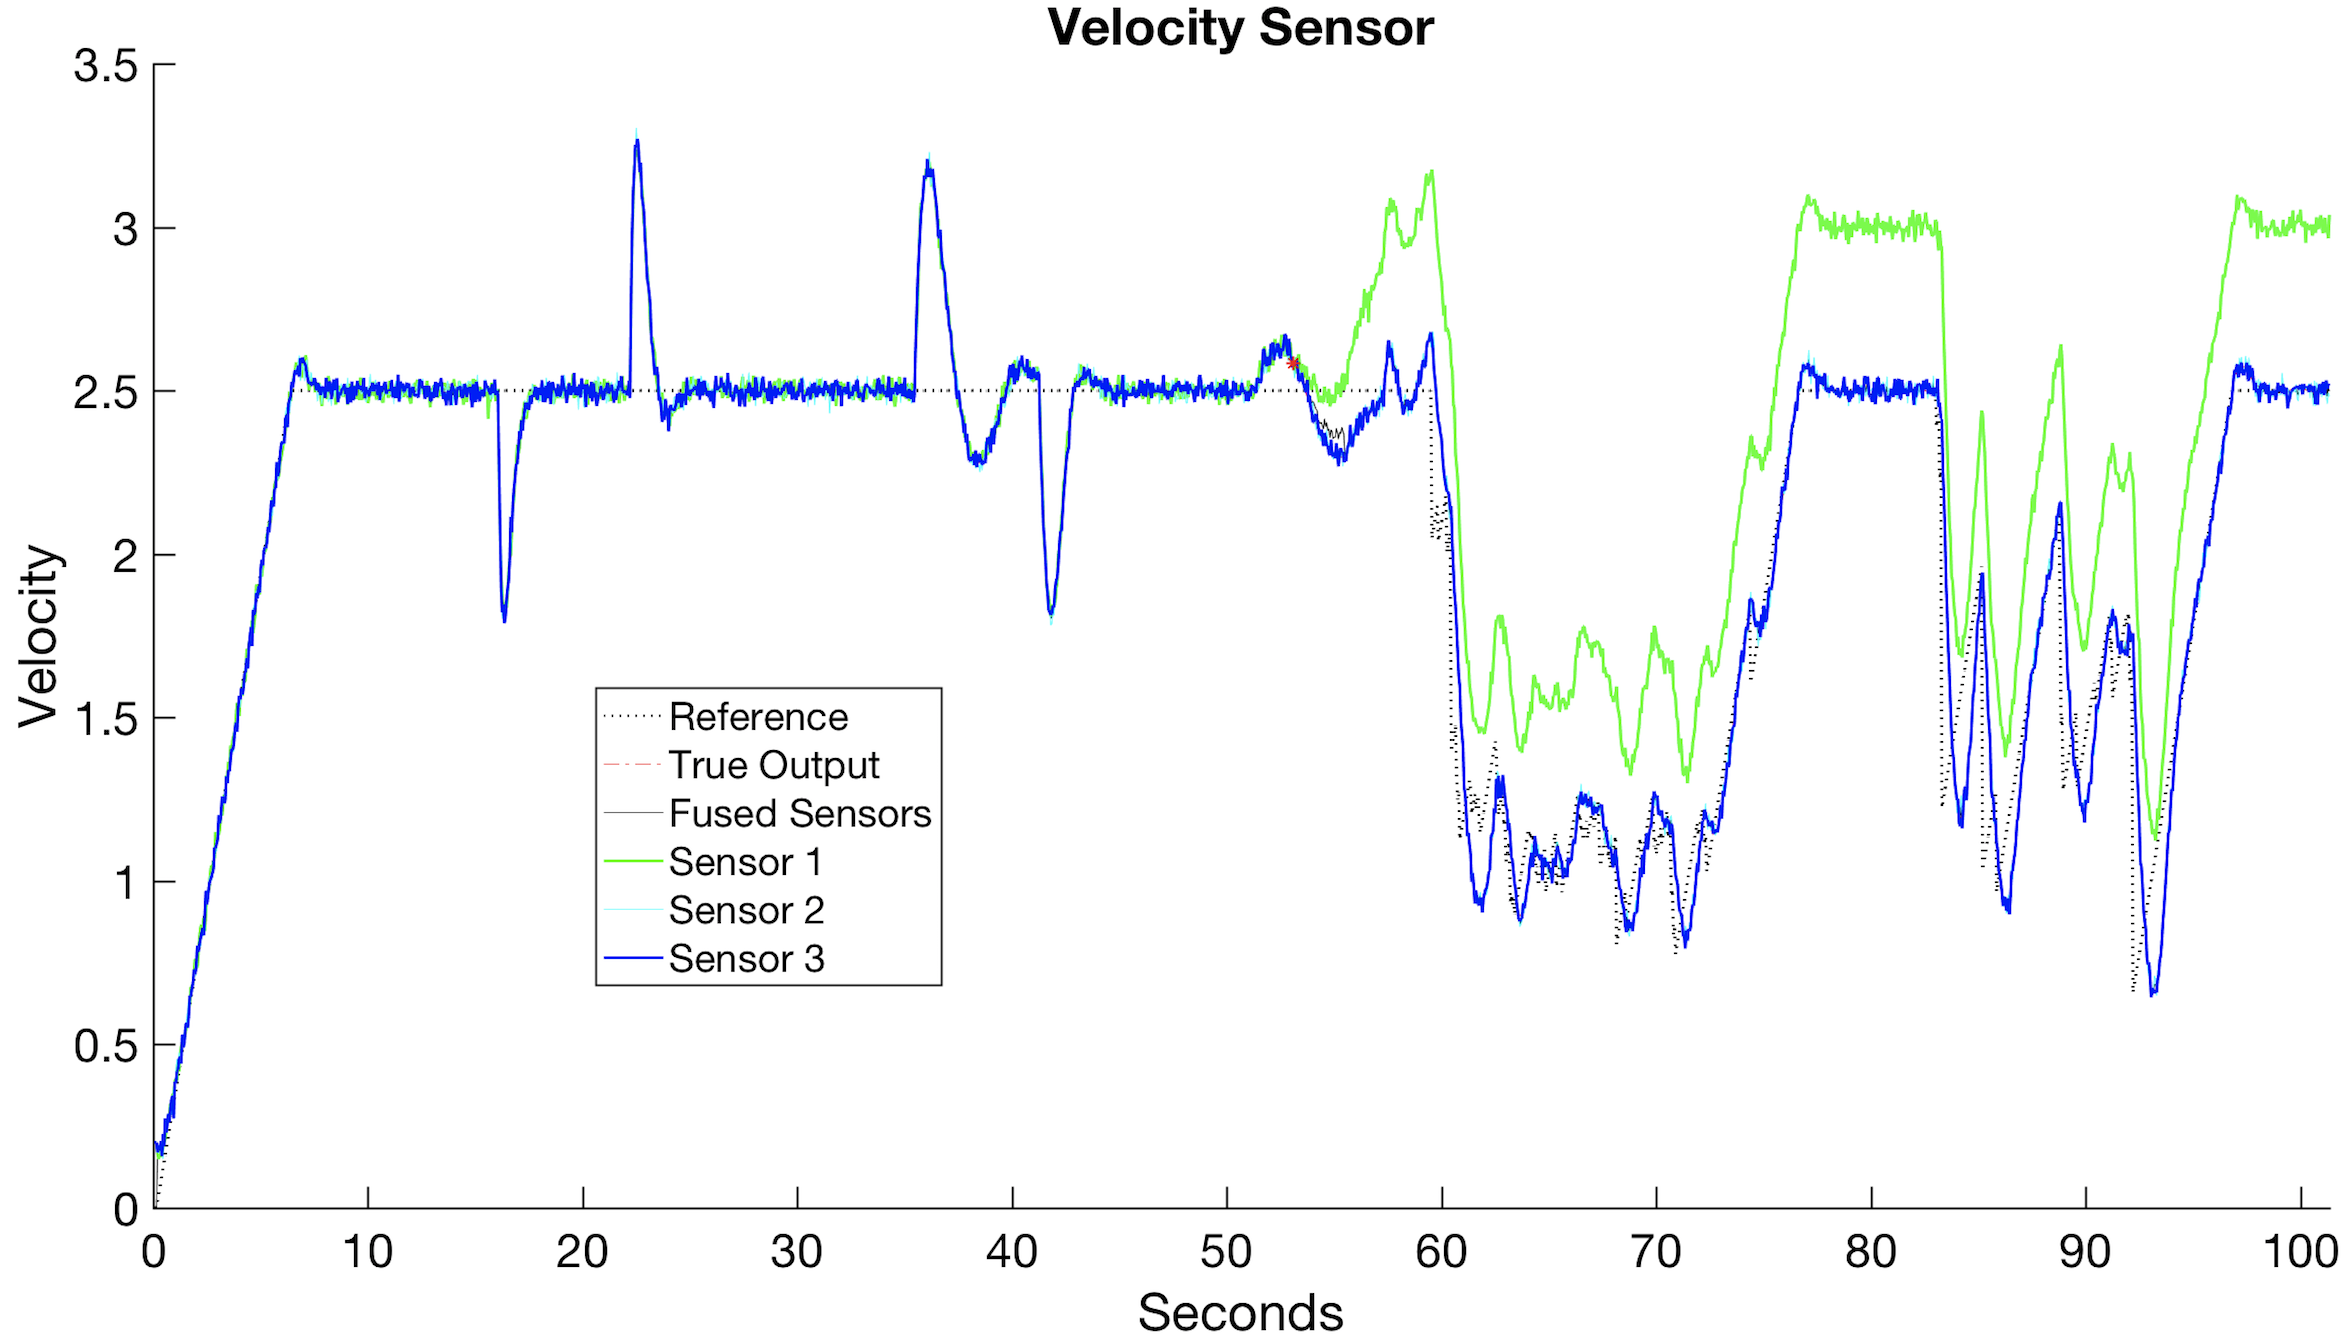
\includegraphics[width=0.48\textwidth]{Figures/Velocities.png}
\caption{Velocities are shown over the entire simulation. Sensor 3 measurements are no longer used by the system as soon as it diverges from the remaining sensors. }
\label{fig:total_velocity}
\end{figure}

In Figure \ref{fig:total_velocity}, the velocity sensors over the entire simulation are displayed. During the time frame between Goals A and C, dynamical changes occur temporarily affecting the velocity tracking. After Goal C, a spoof on Sensor 1 causing it diverge from the other sensors. The detector removes the compromised sensor, allowing the system to maintain reference tracking.


\begin{figure}[ht!]
\centering
\begin{tabular}{cc}
\subfigure[\label{fig:MRAC_tracking} ]{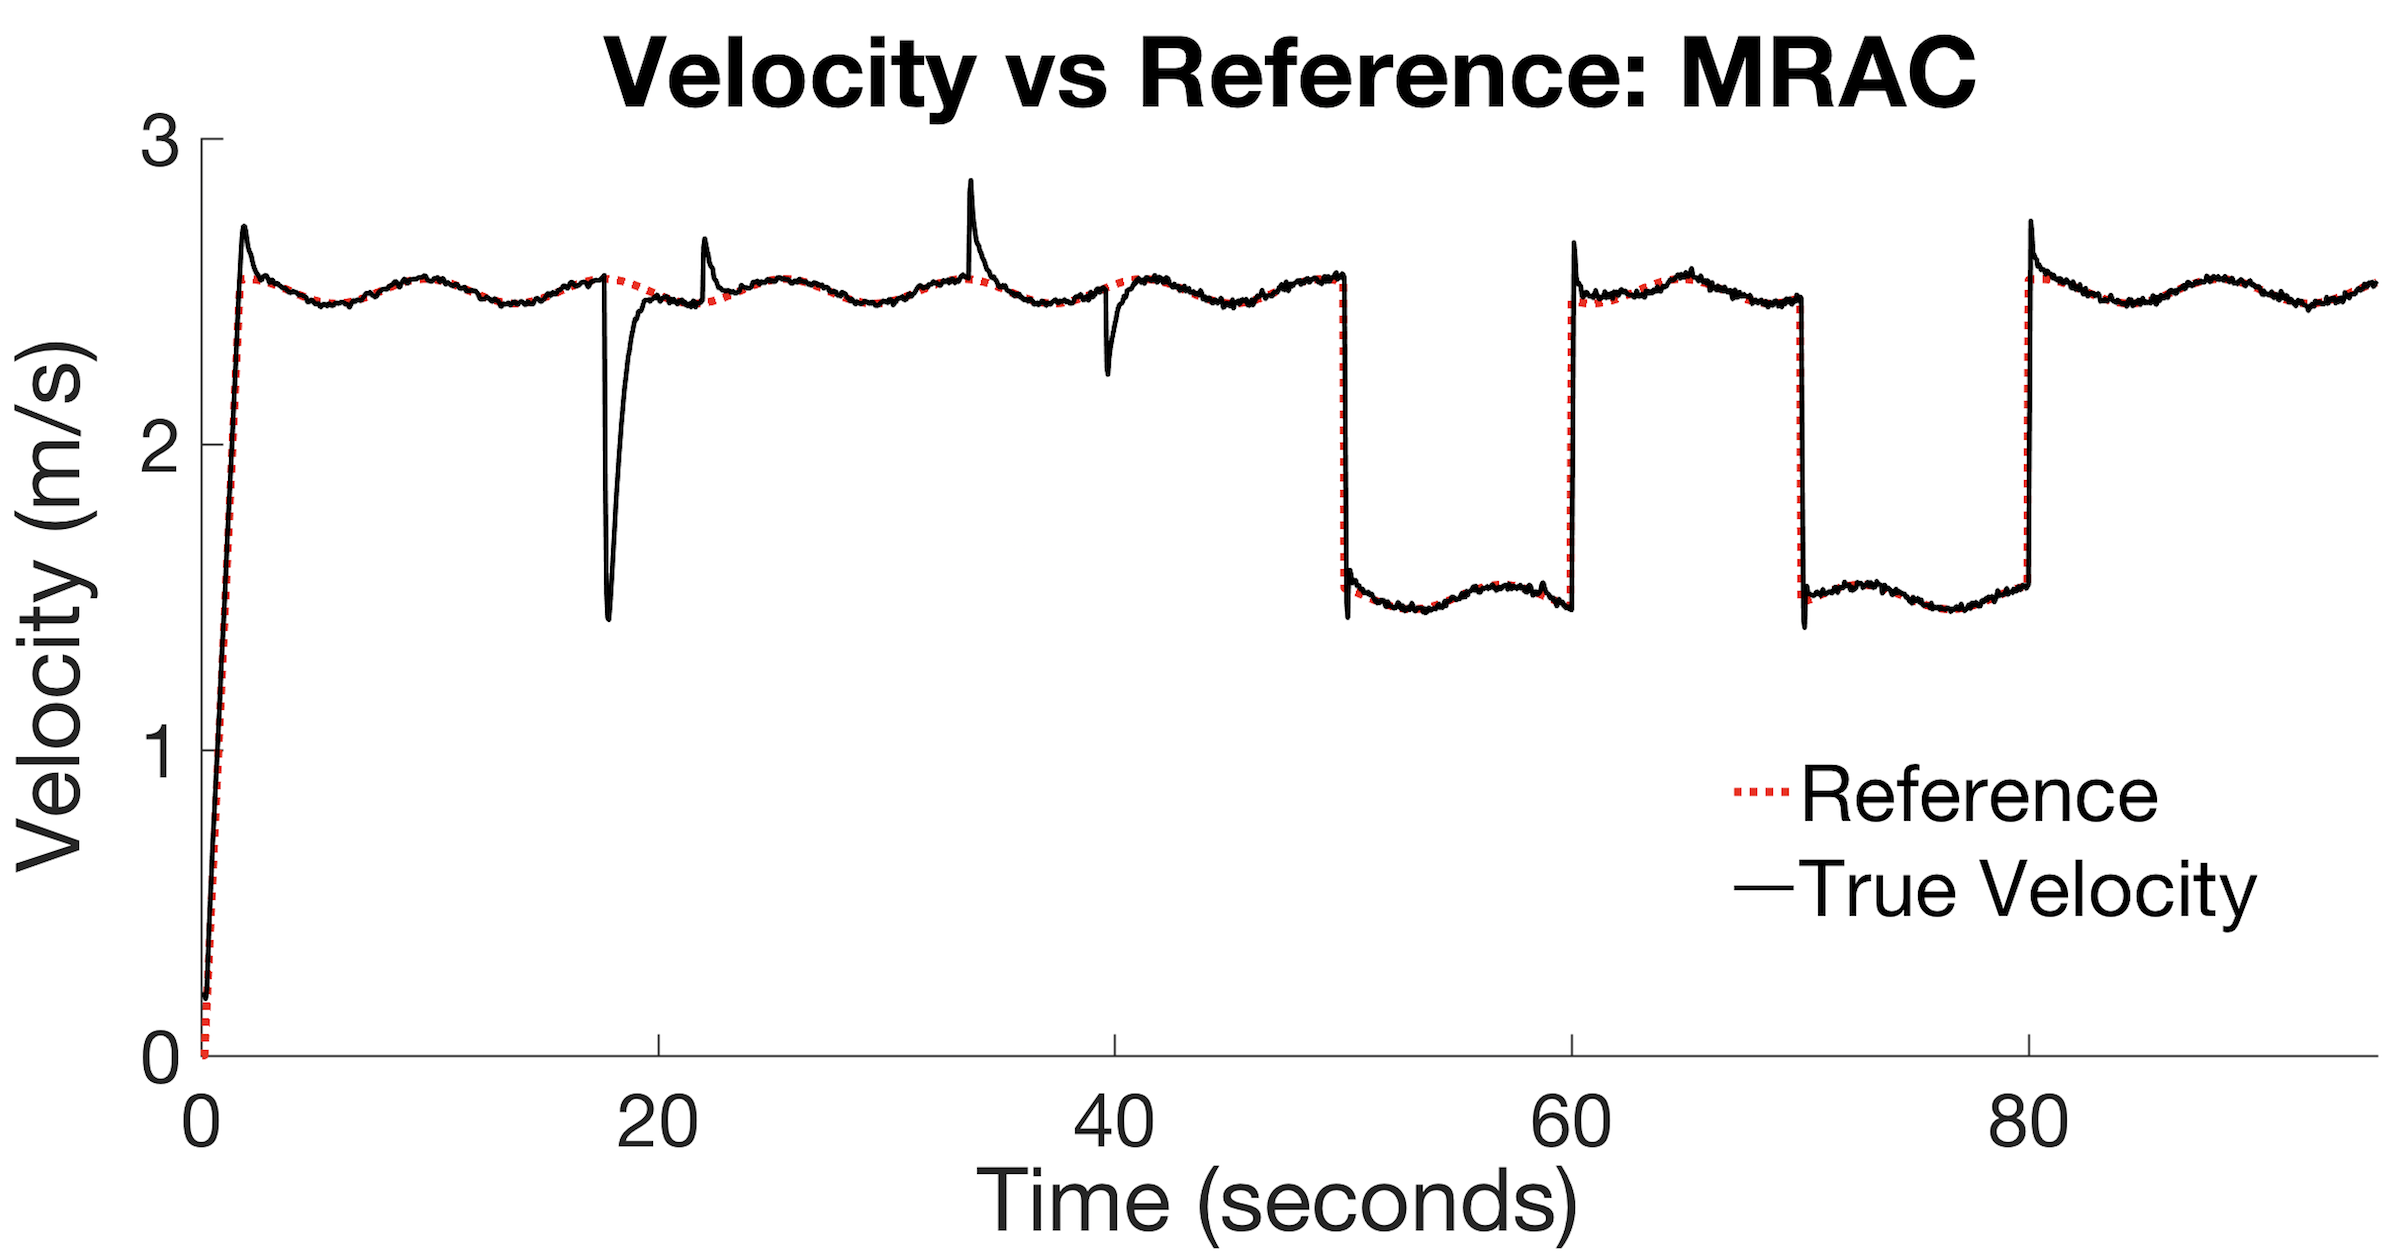
\includegraphics[width = 0.22\textwidth]{Figures/VelocityTracking_MRAC.png}} & 
\subfigure[\label{fig:PID_tracking} ]{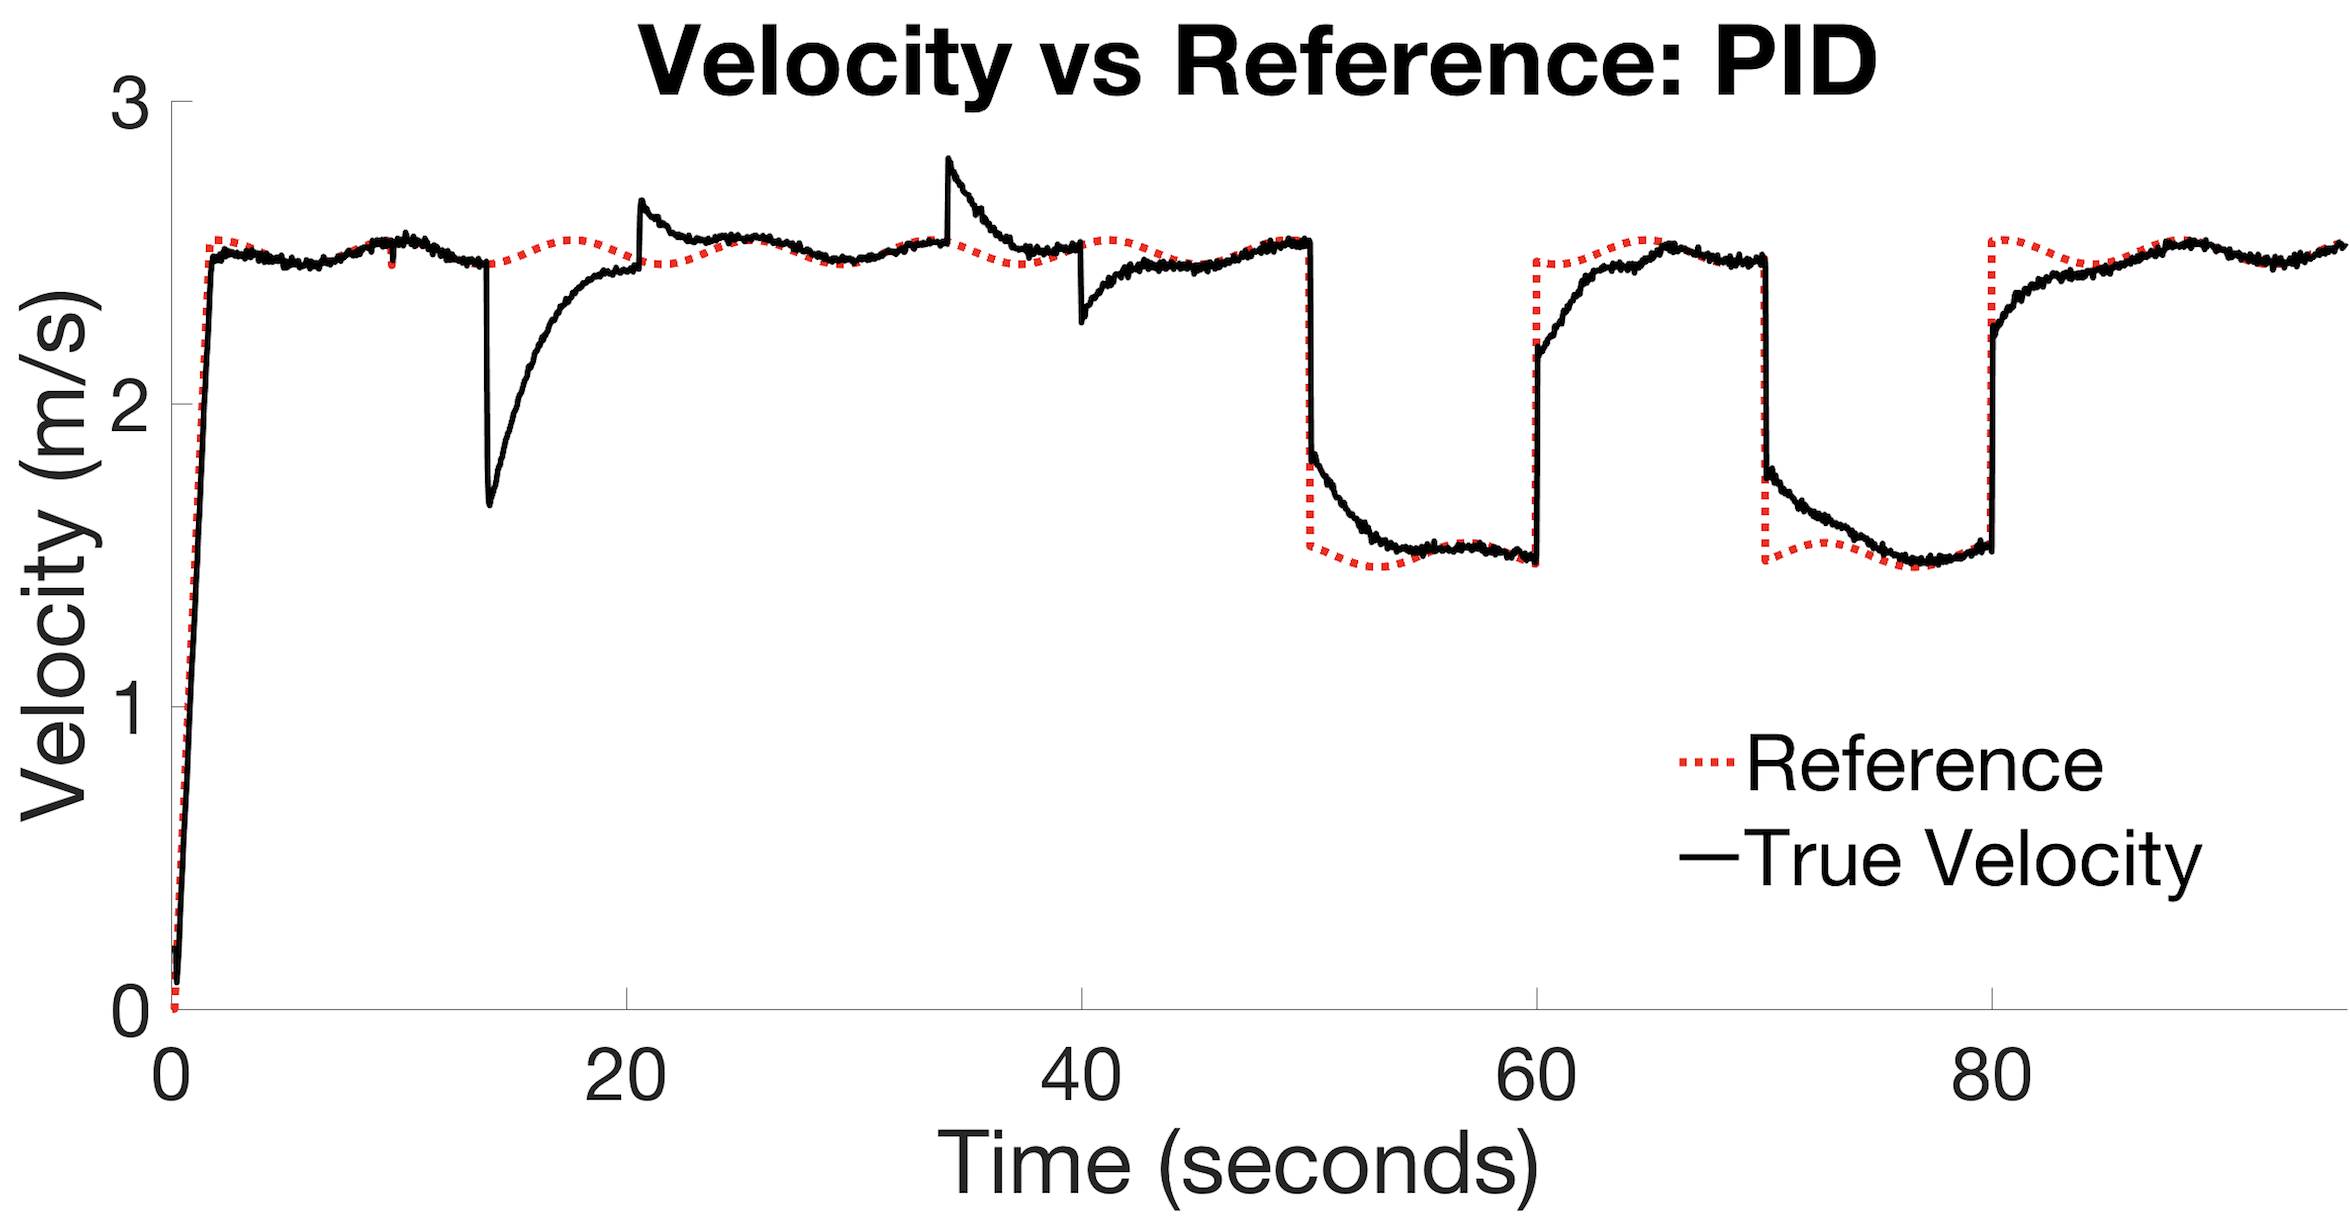
\includegraphics[width =0.22\textwidth]{Figures/VelocityTracking_PID.png}}
\end{tabular}
\label{fig:ControllerComparisons}
\caption{A performance comparison between the model reference adaptive controller (MRAC) vs Proportional-Integral-Derivative (PID) controller tuned for the initial model.}
\end{figure}

A comparison of control performance in Figure \ref{fig:ControllerComparisons} shows the benefits of the adaptive controller. As dynamics change away from the initial model, the PID controller loses control performance in which the tracking convergence is degraded.




\begin{figure}
\vspace{1pt}
%\centering
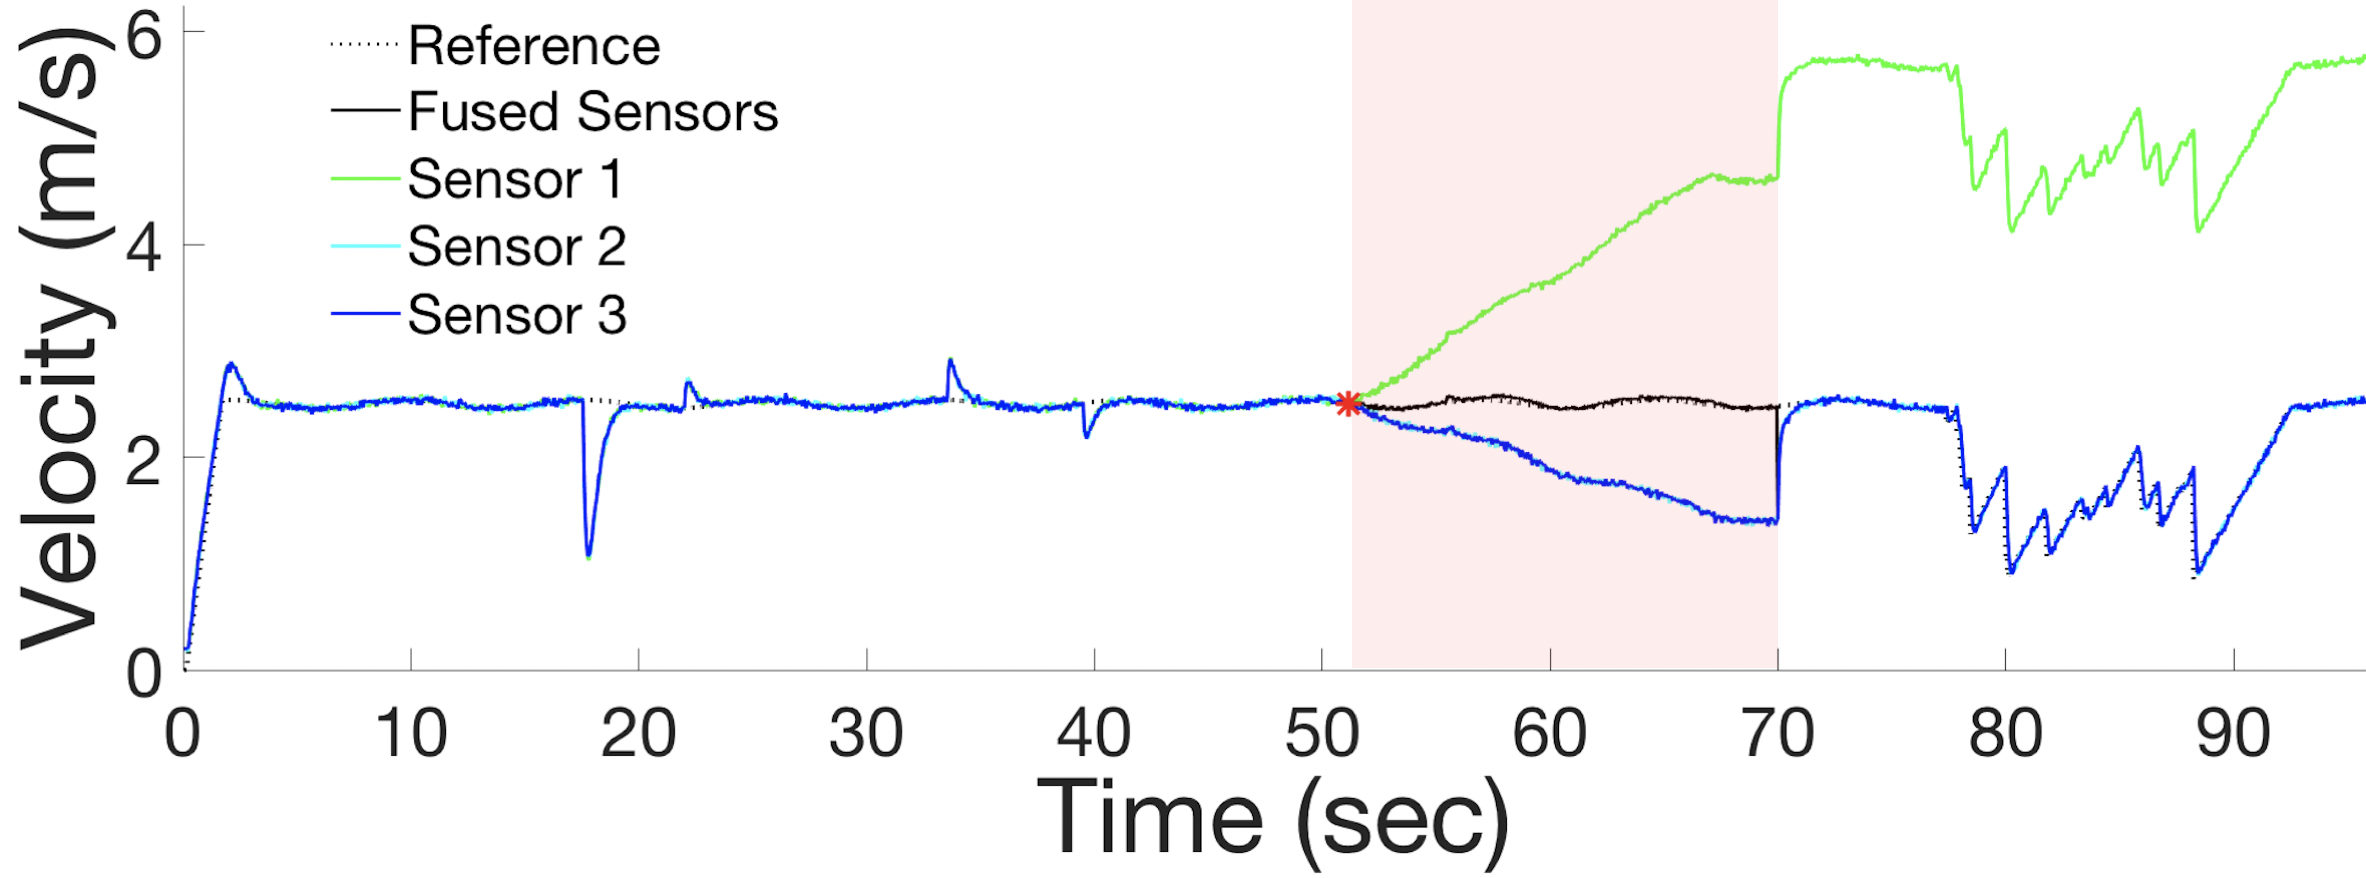
\includegraphics[width = 0.48\textwidth]{Figures/NoDetection_Vel.png}
\caption{A demonstration of an attack with the detector not operating for a period of time during an attack. }
\label{fig:NoDet_Vel}
\end{figure}

Figure \ref{fig:NoDet_Vel} shows a time frame of the detector turned off, where an attacker is free to compromise the system. A ramp attack is performed, slowly pushing a sensor away from the true value. The red shaded region is the time frame the attack occurred without the attack detector operating. As the right shaded region ends, the detector is turned on and the sensor is removed.


\begin{figure}
%\begin{figure*}[th!]
\begin{tabular}{cc}

\subfigure[\label{fig:error_comp1} ]{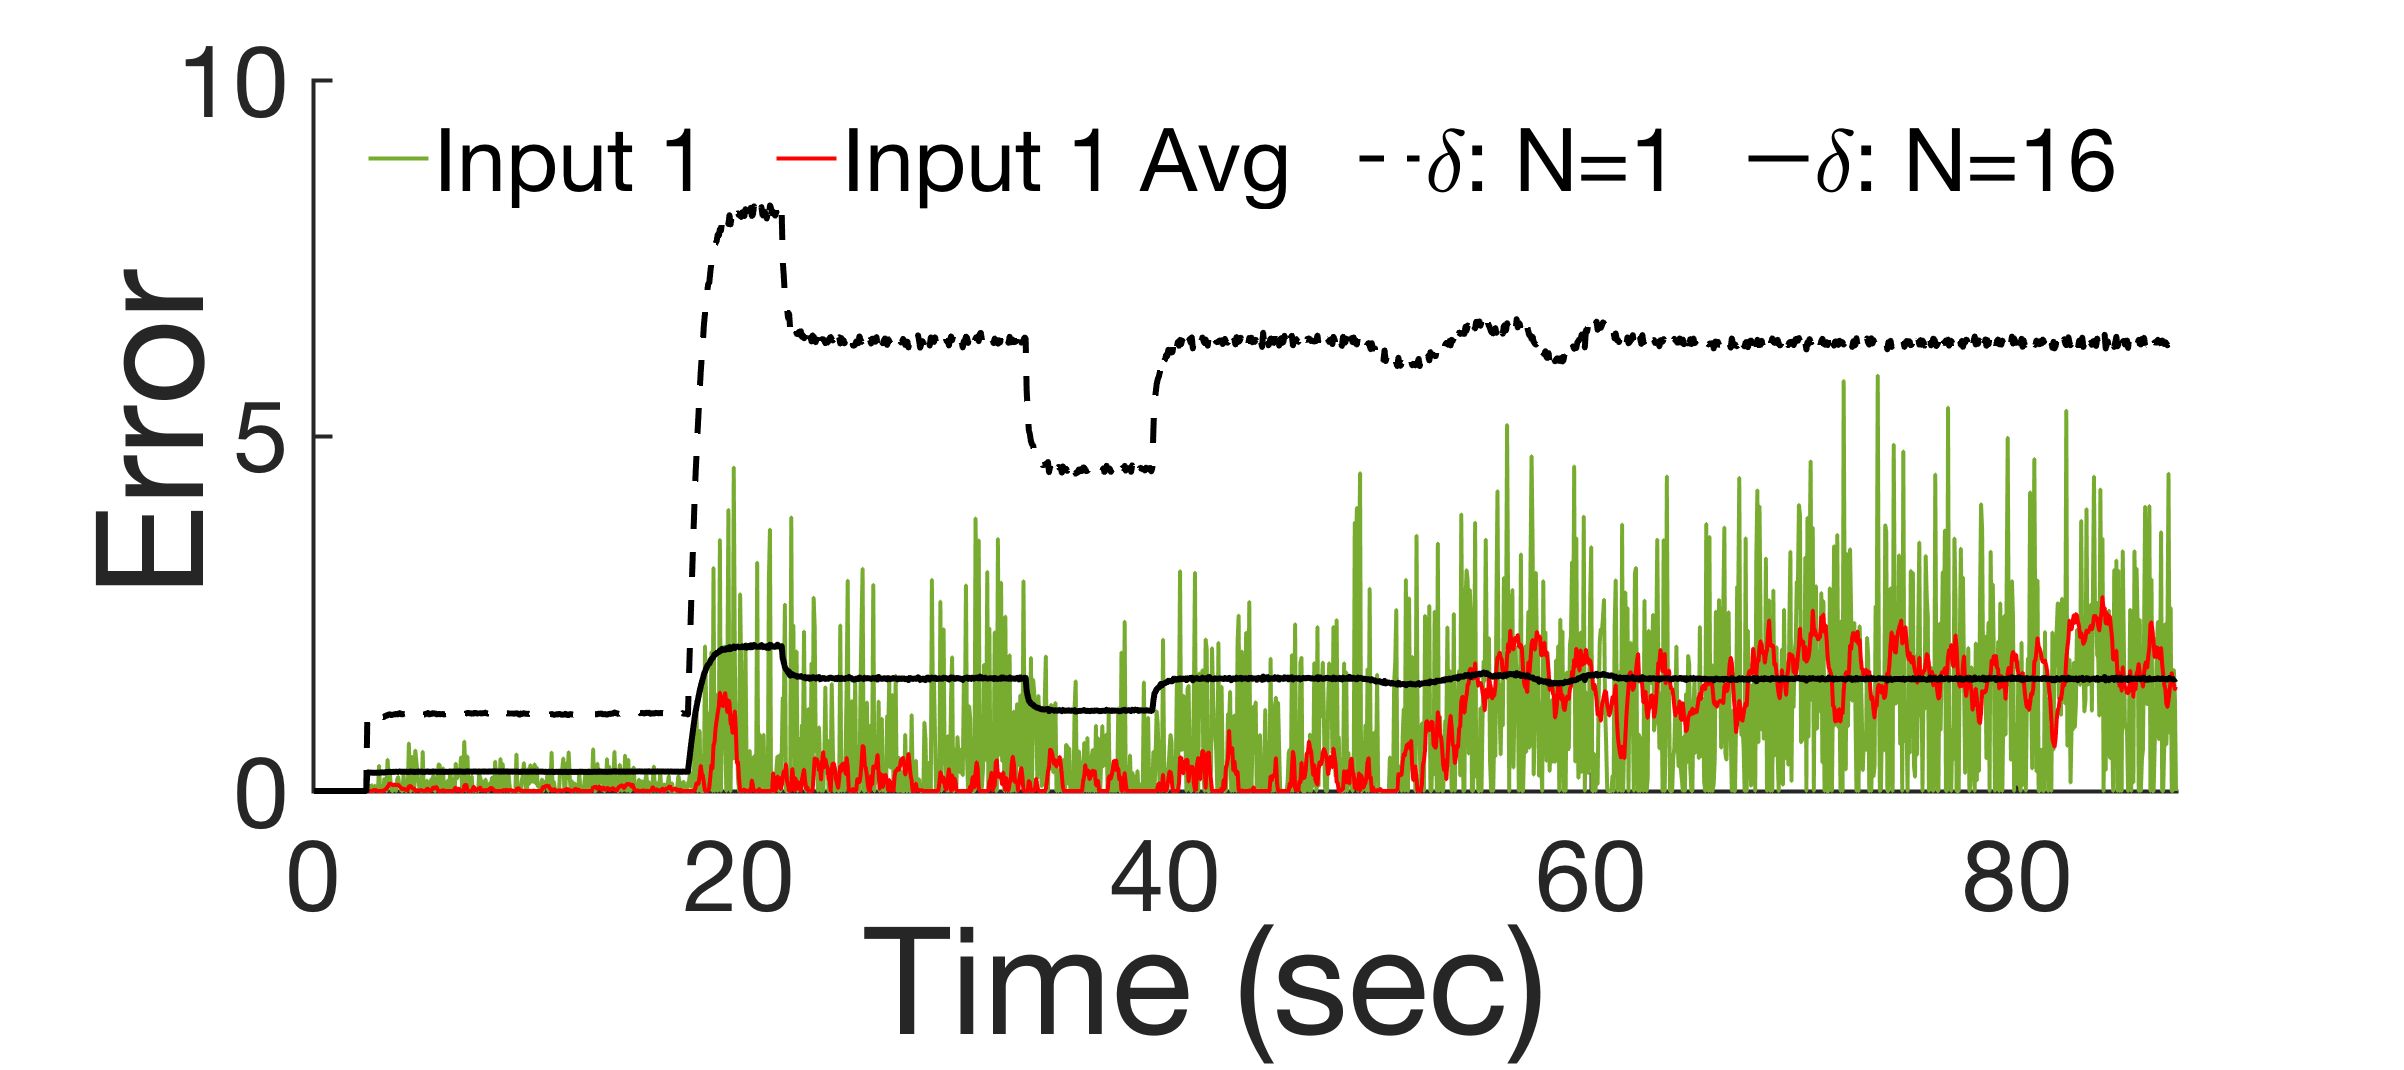
\includegraphics[width = 0.22\textwidth]{Figures/ErrorComparison1.png}} &	
\subfigure[\label{fig:error_comp2} ]{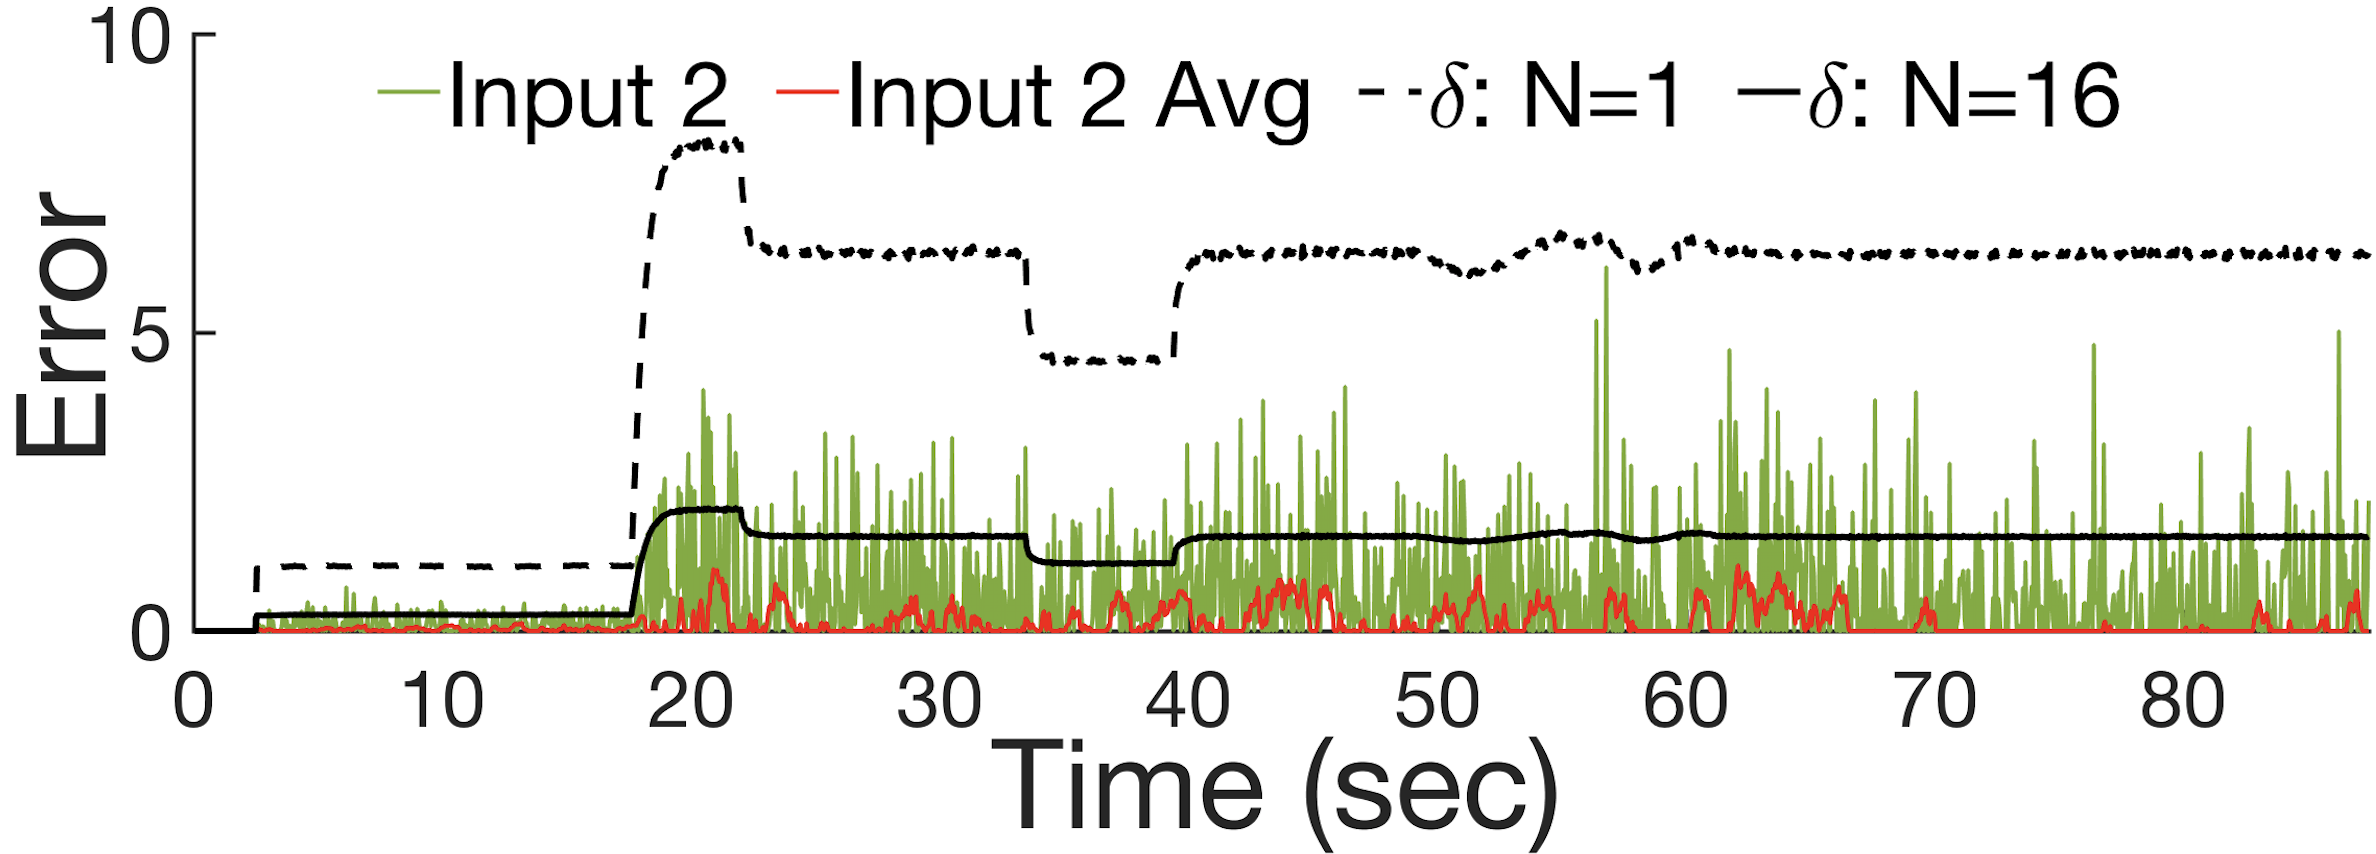
\includegraphics[width = 0.22\textwidth]{Figures/ErrorComparison2.png}}
\end{tabular} \\
\begin{tabular}{cc}
\subfigure[\label{fig:error_comp3} ]{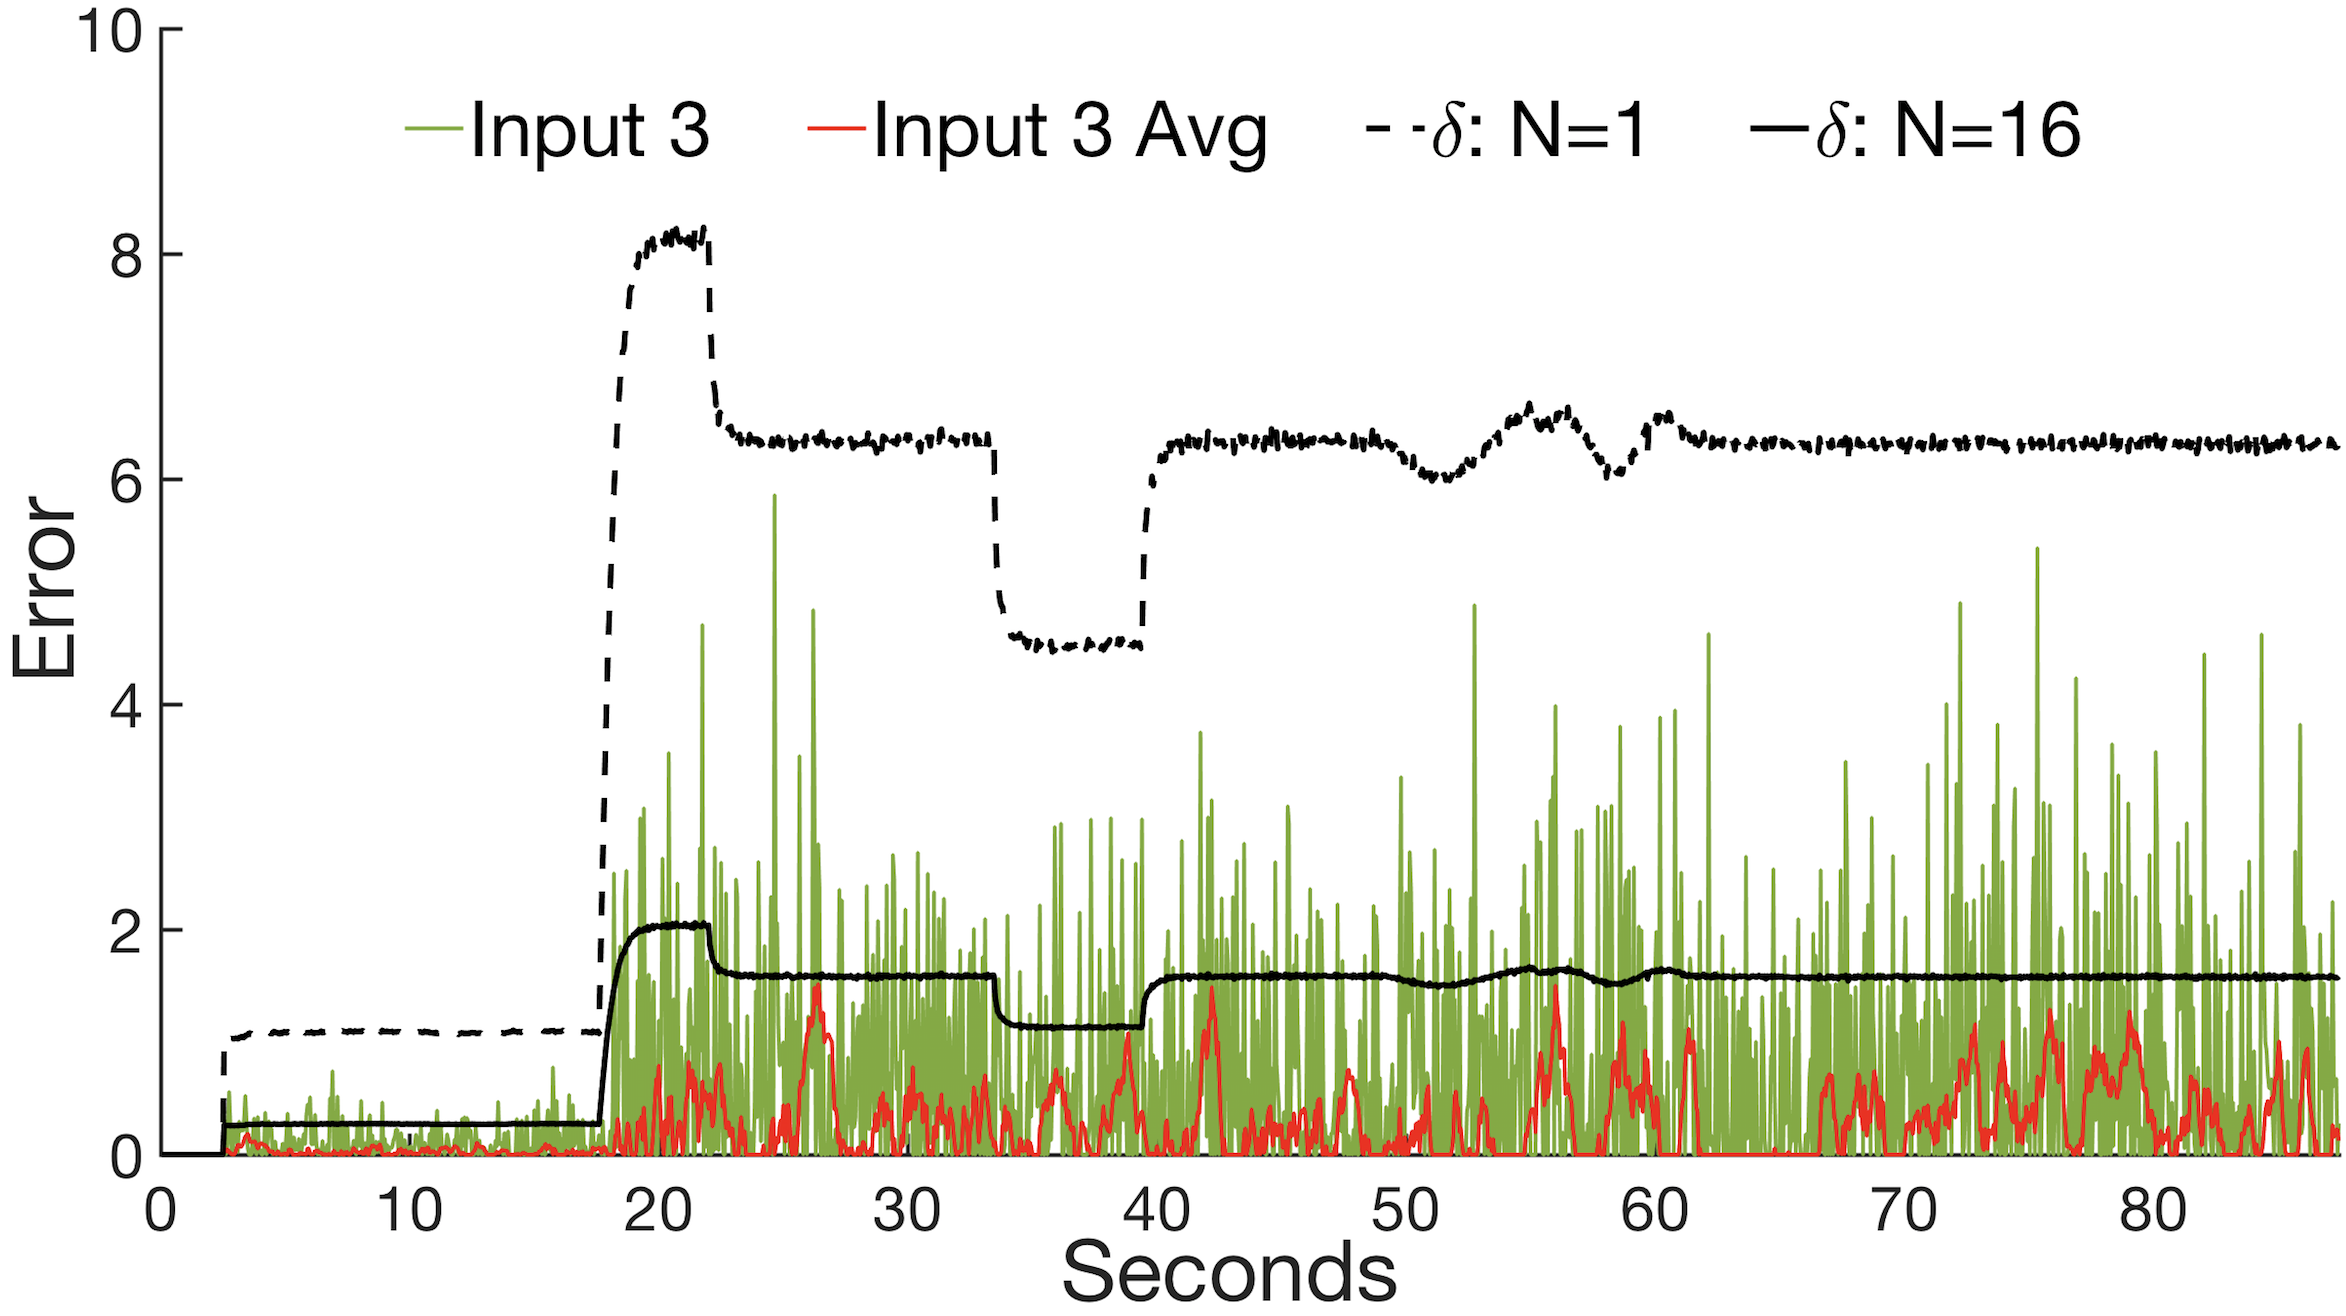
\includegraphics[width = 0.22\textwidth]{Figures/ErrorComparison3.png}} &
\subfigure[\label{fig:error_comp4} ]{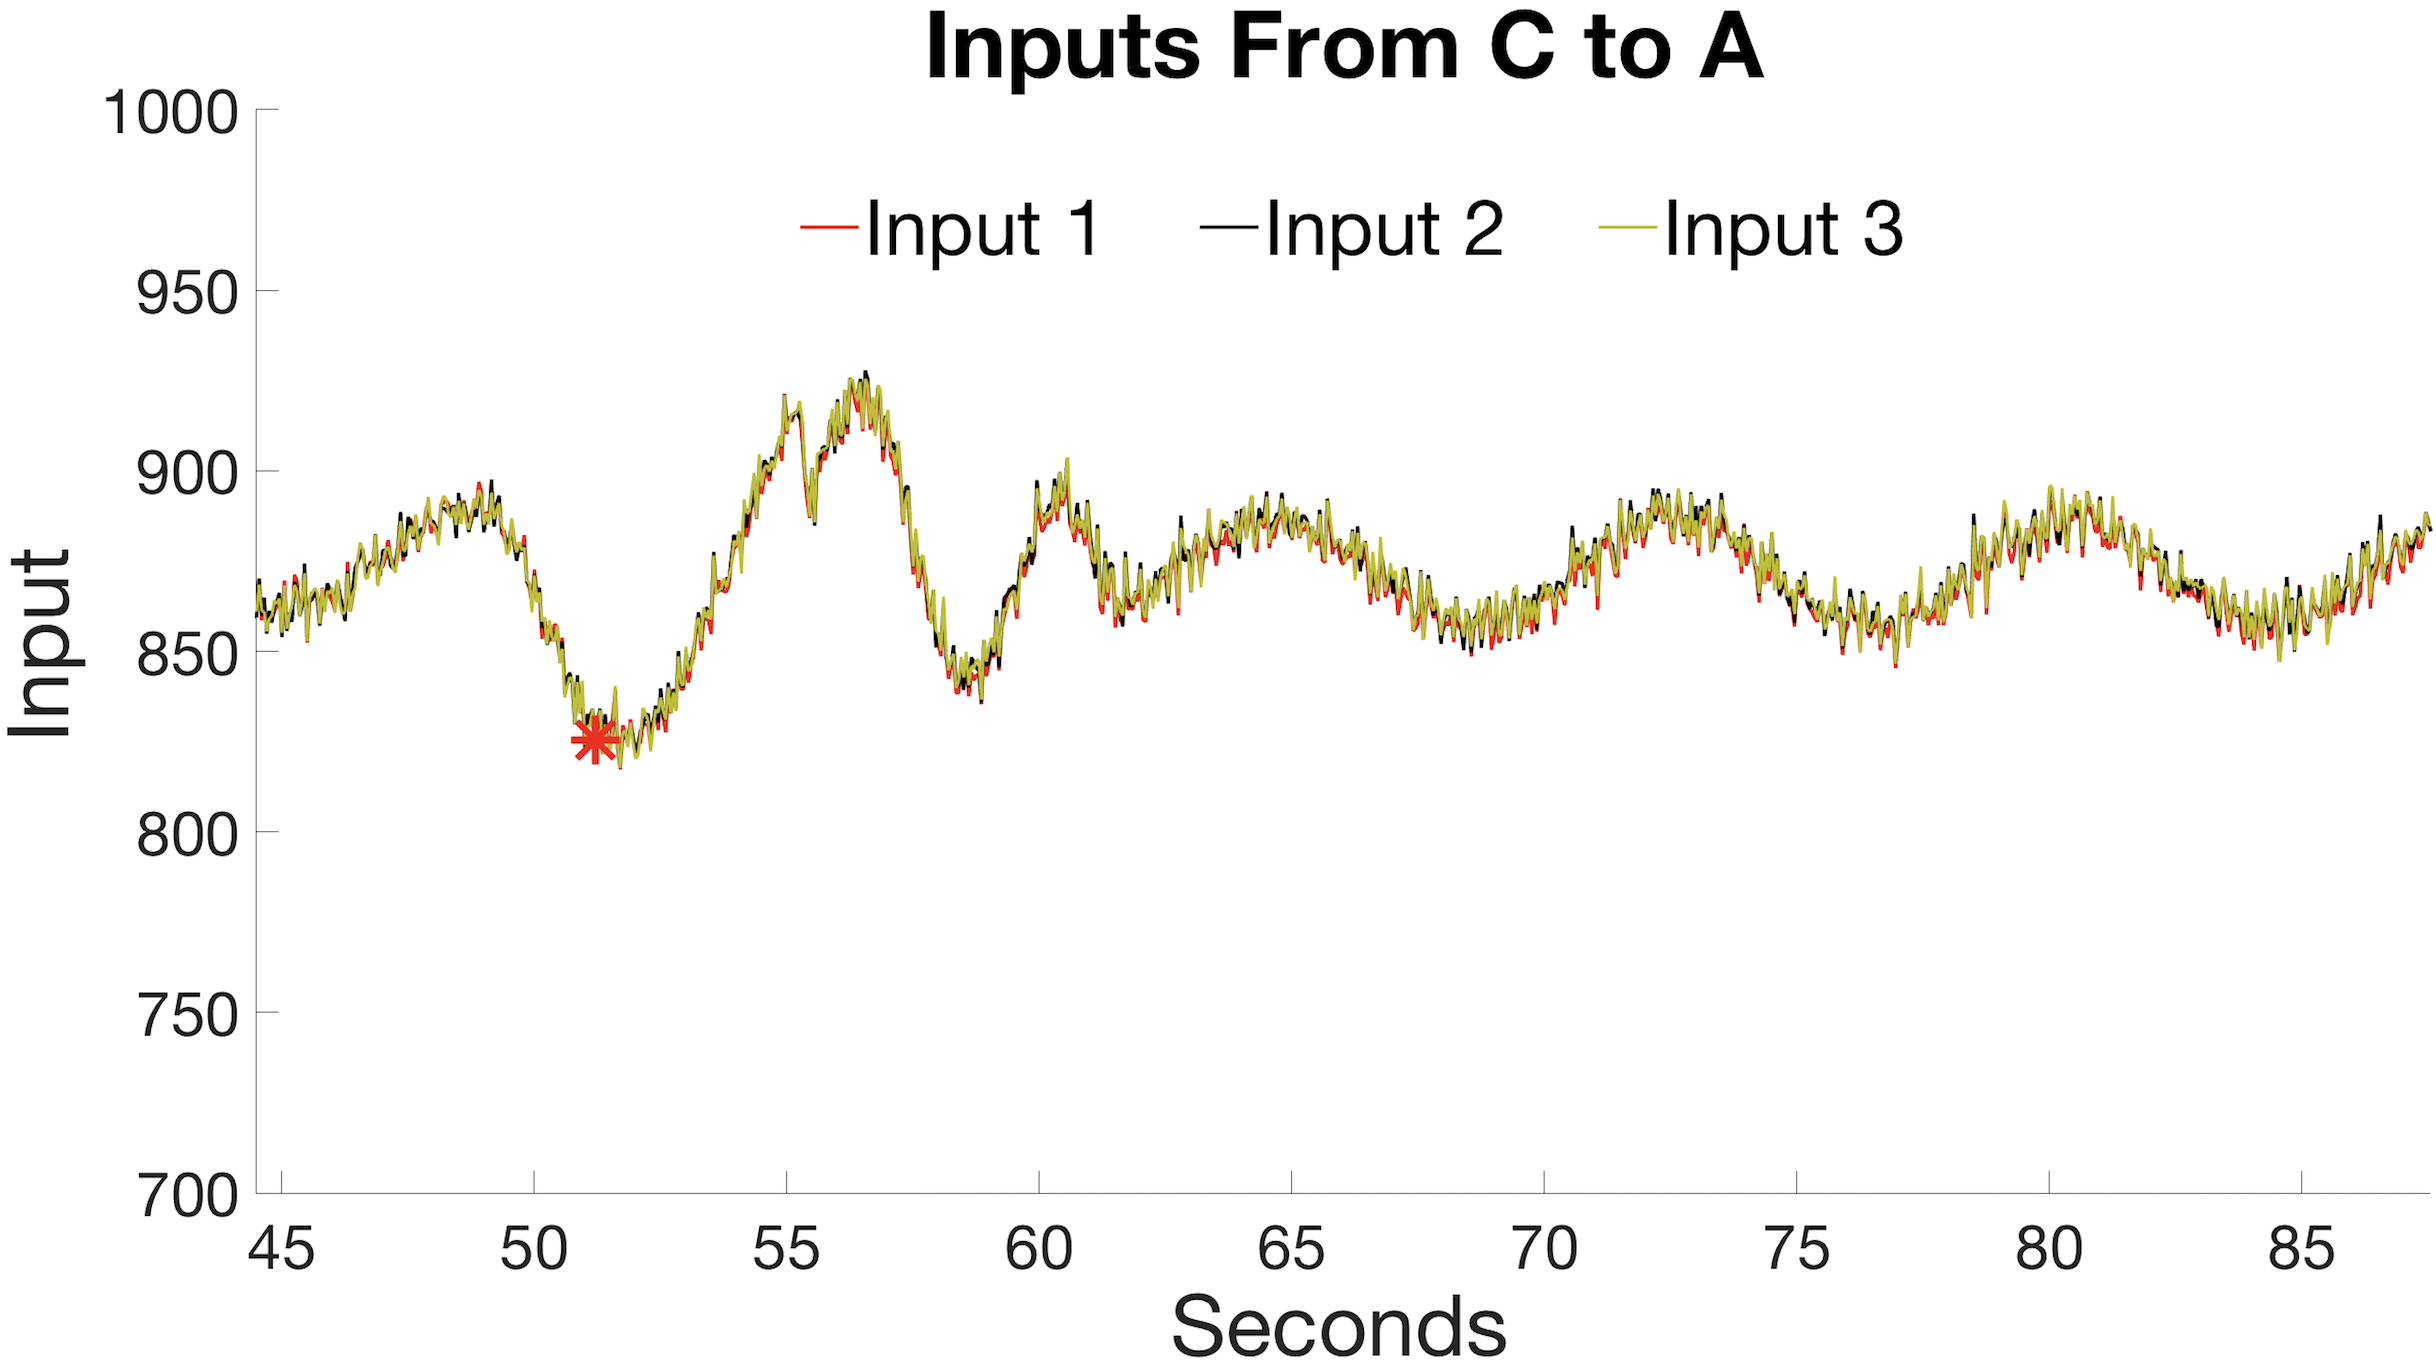
\includegraphics[width = 0.22\textwidth]{Figures/ErrorComparison4.png}}

\end{tabular}
\caption{An attacker performing a stealthy attack within the noise profile. As shown in (a),(b), and (c), the threshold $\delta$ is reduced when averaging the past $N_p$ input values. }

\label{fig:Stealthy_Attack}
\end{figure}

Stealthy attacks within the sensor noise profile can be detected by using more input values to reduce the noise threshold $\delta$. The case in Figure \ref{fig:Stealthy_Attack} demonstrates the attack on Sensor 1 is detected when using $N_p=16$ input values, but would have never been detected when $N_p=1$ as the error stayed below the error threshold $\delta$.


\end{section}